% !TEX root = ../report.tex
\section*{Techniques}\label{sec:techniques}
\addcontentsline{toc}{section}{Techniques}

\begin{figure}[H]
	\subfloat[]{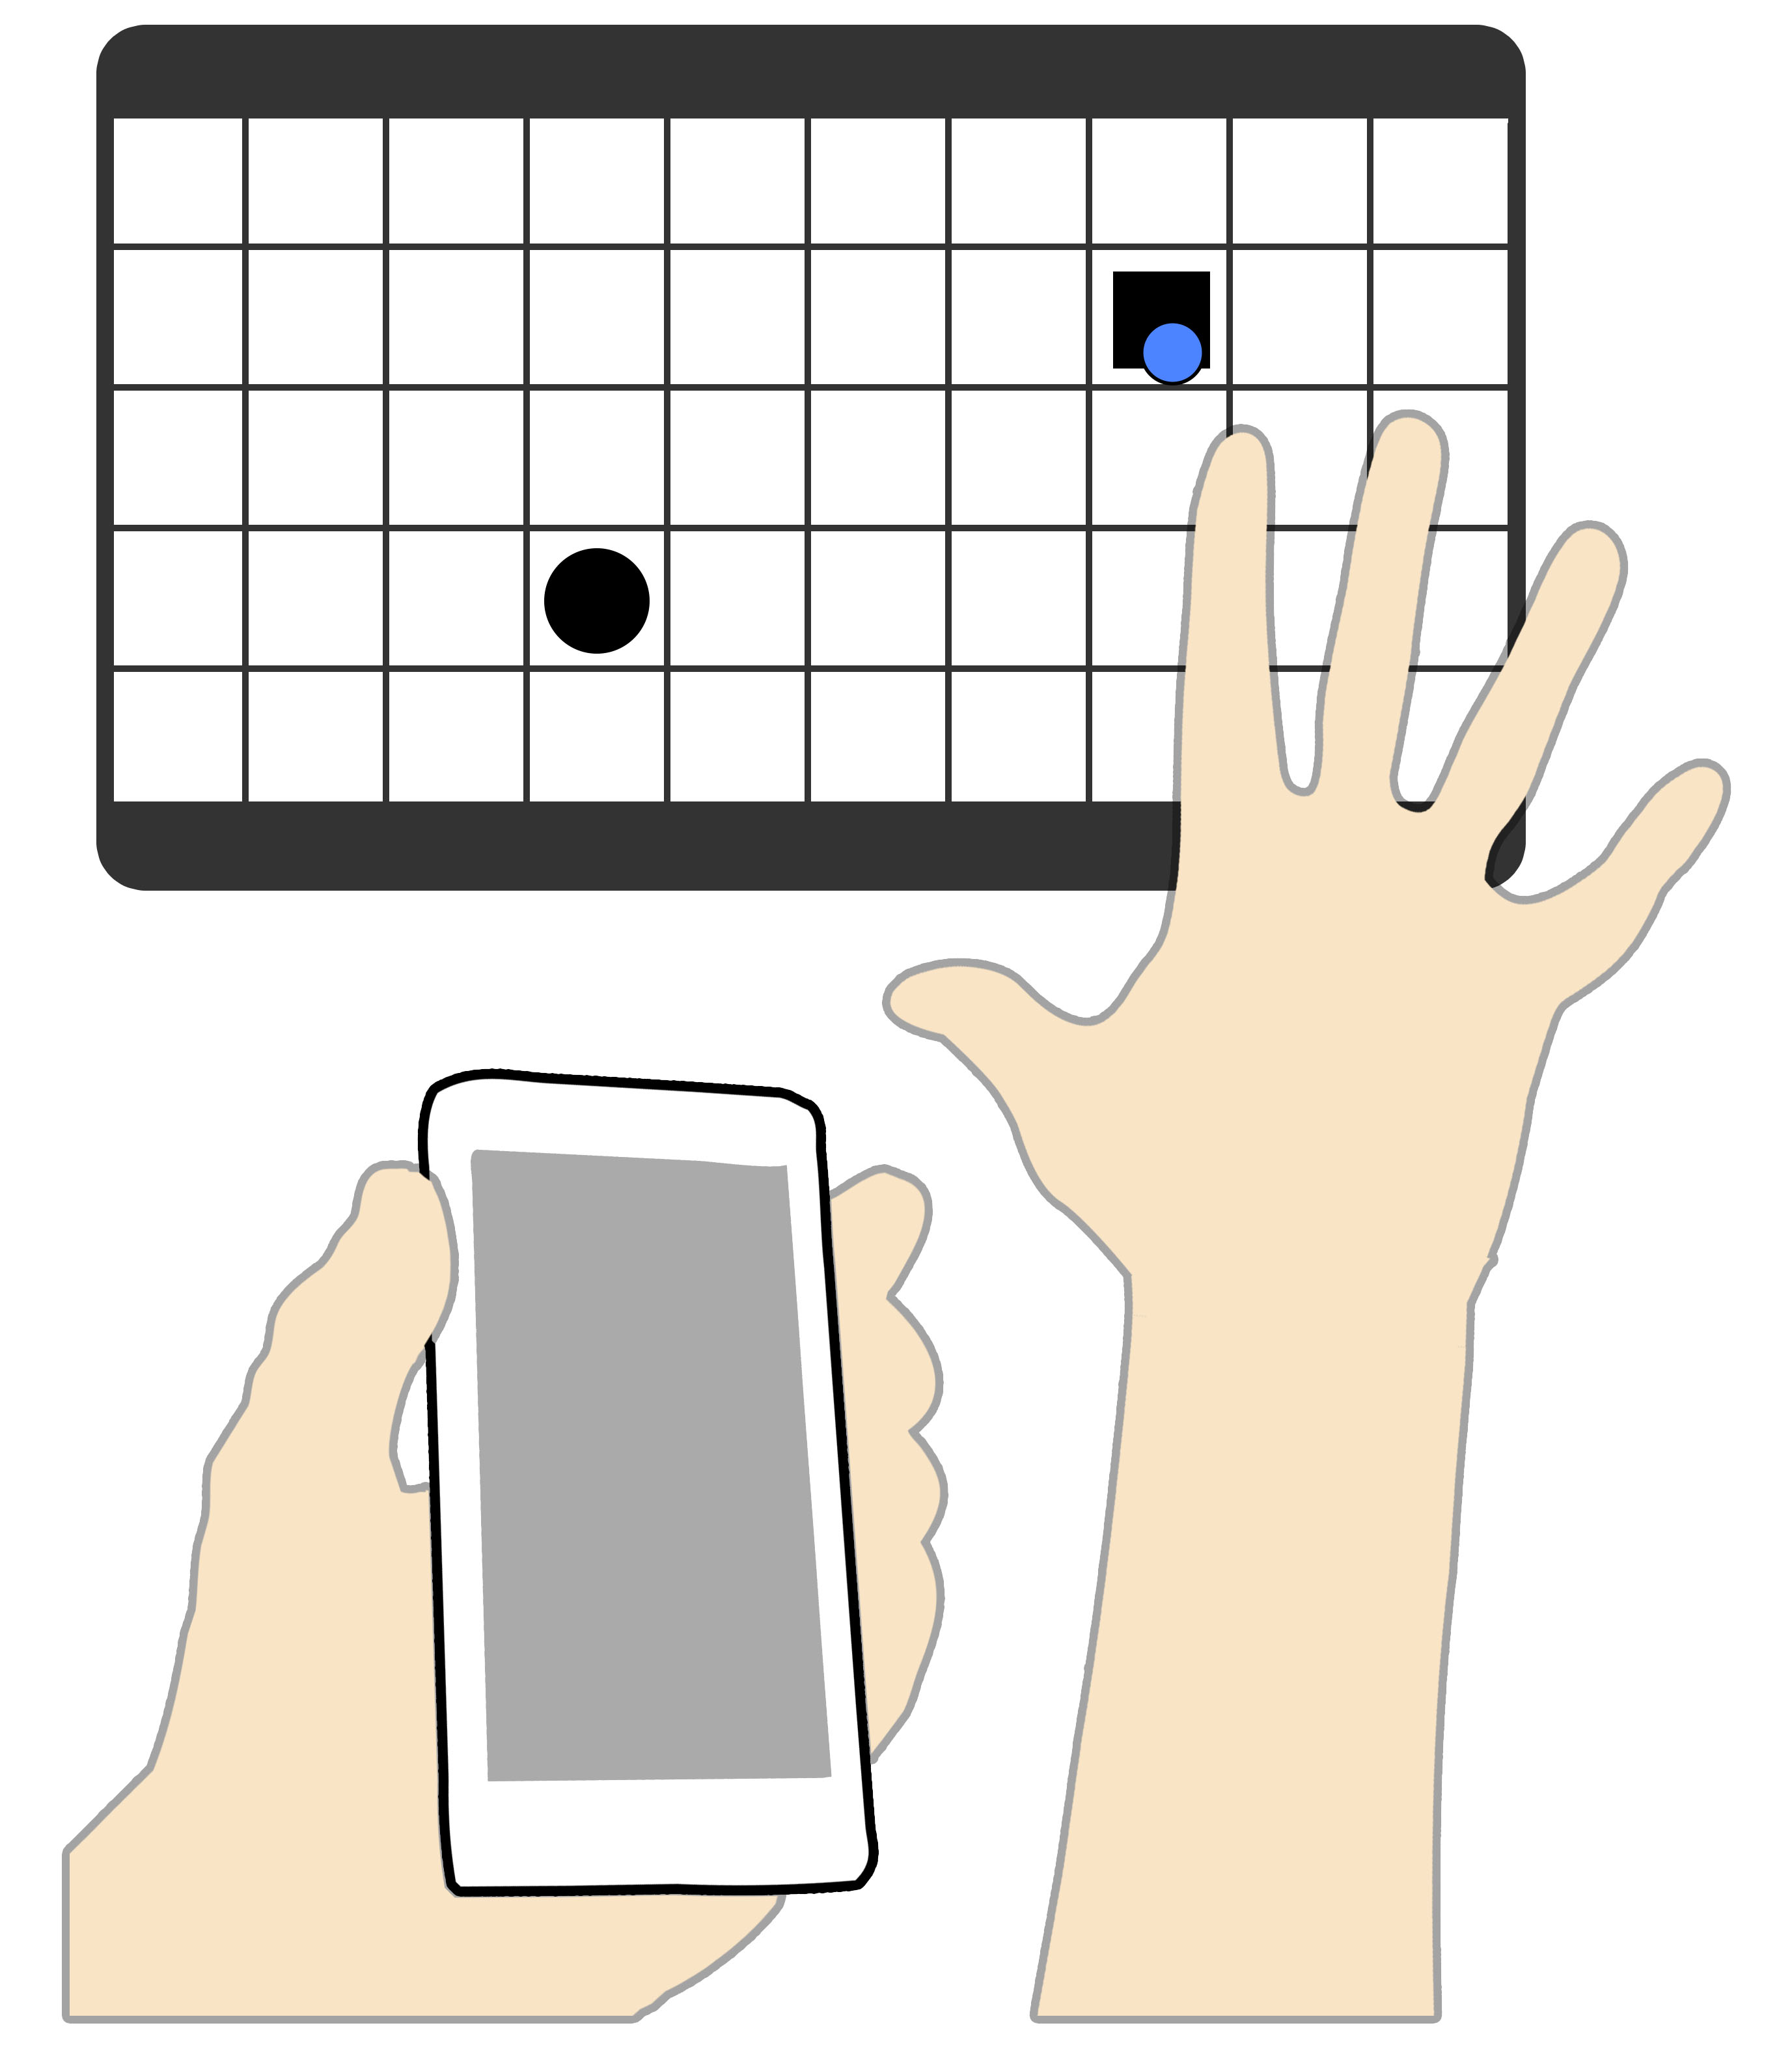
\includegraphics[width = 0.33\columnwidth]{images/techniques/grabPull1.jpg}\label{fig:grabPull1}}
	\subfloat[]{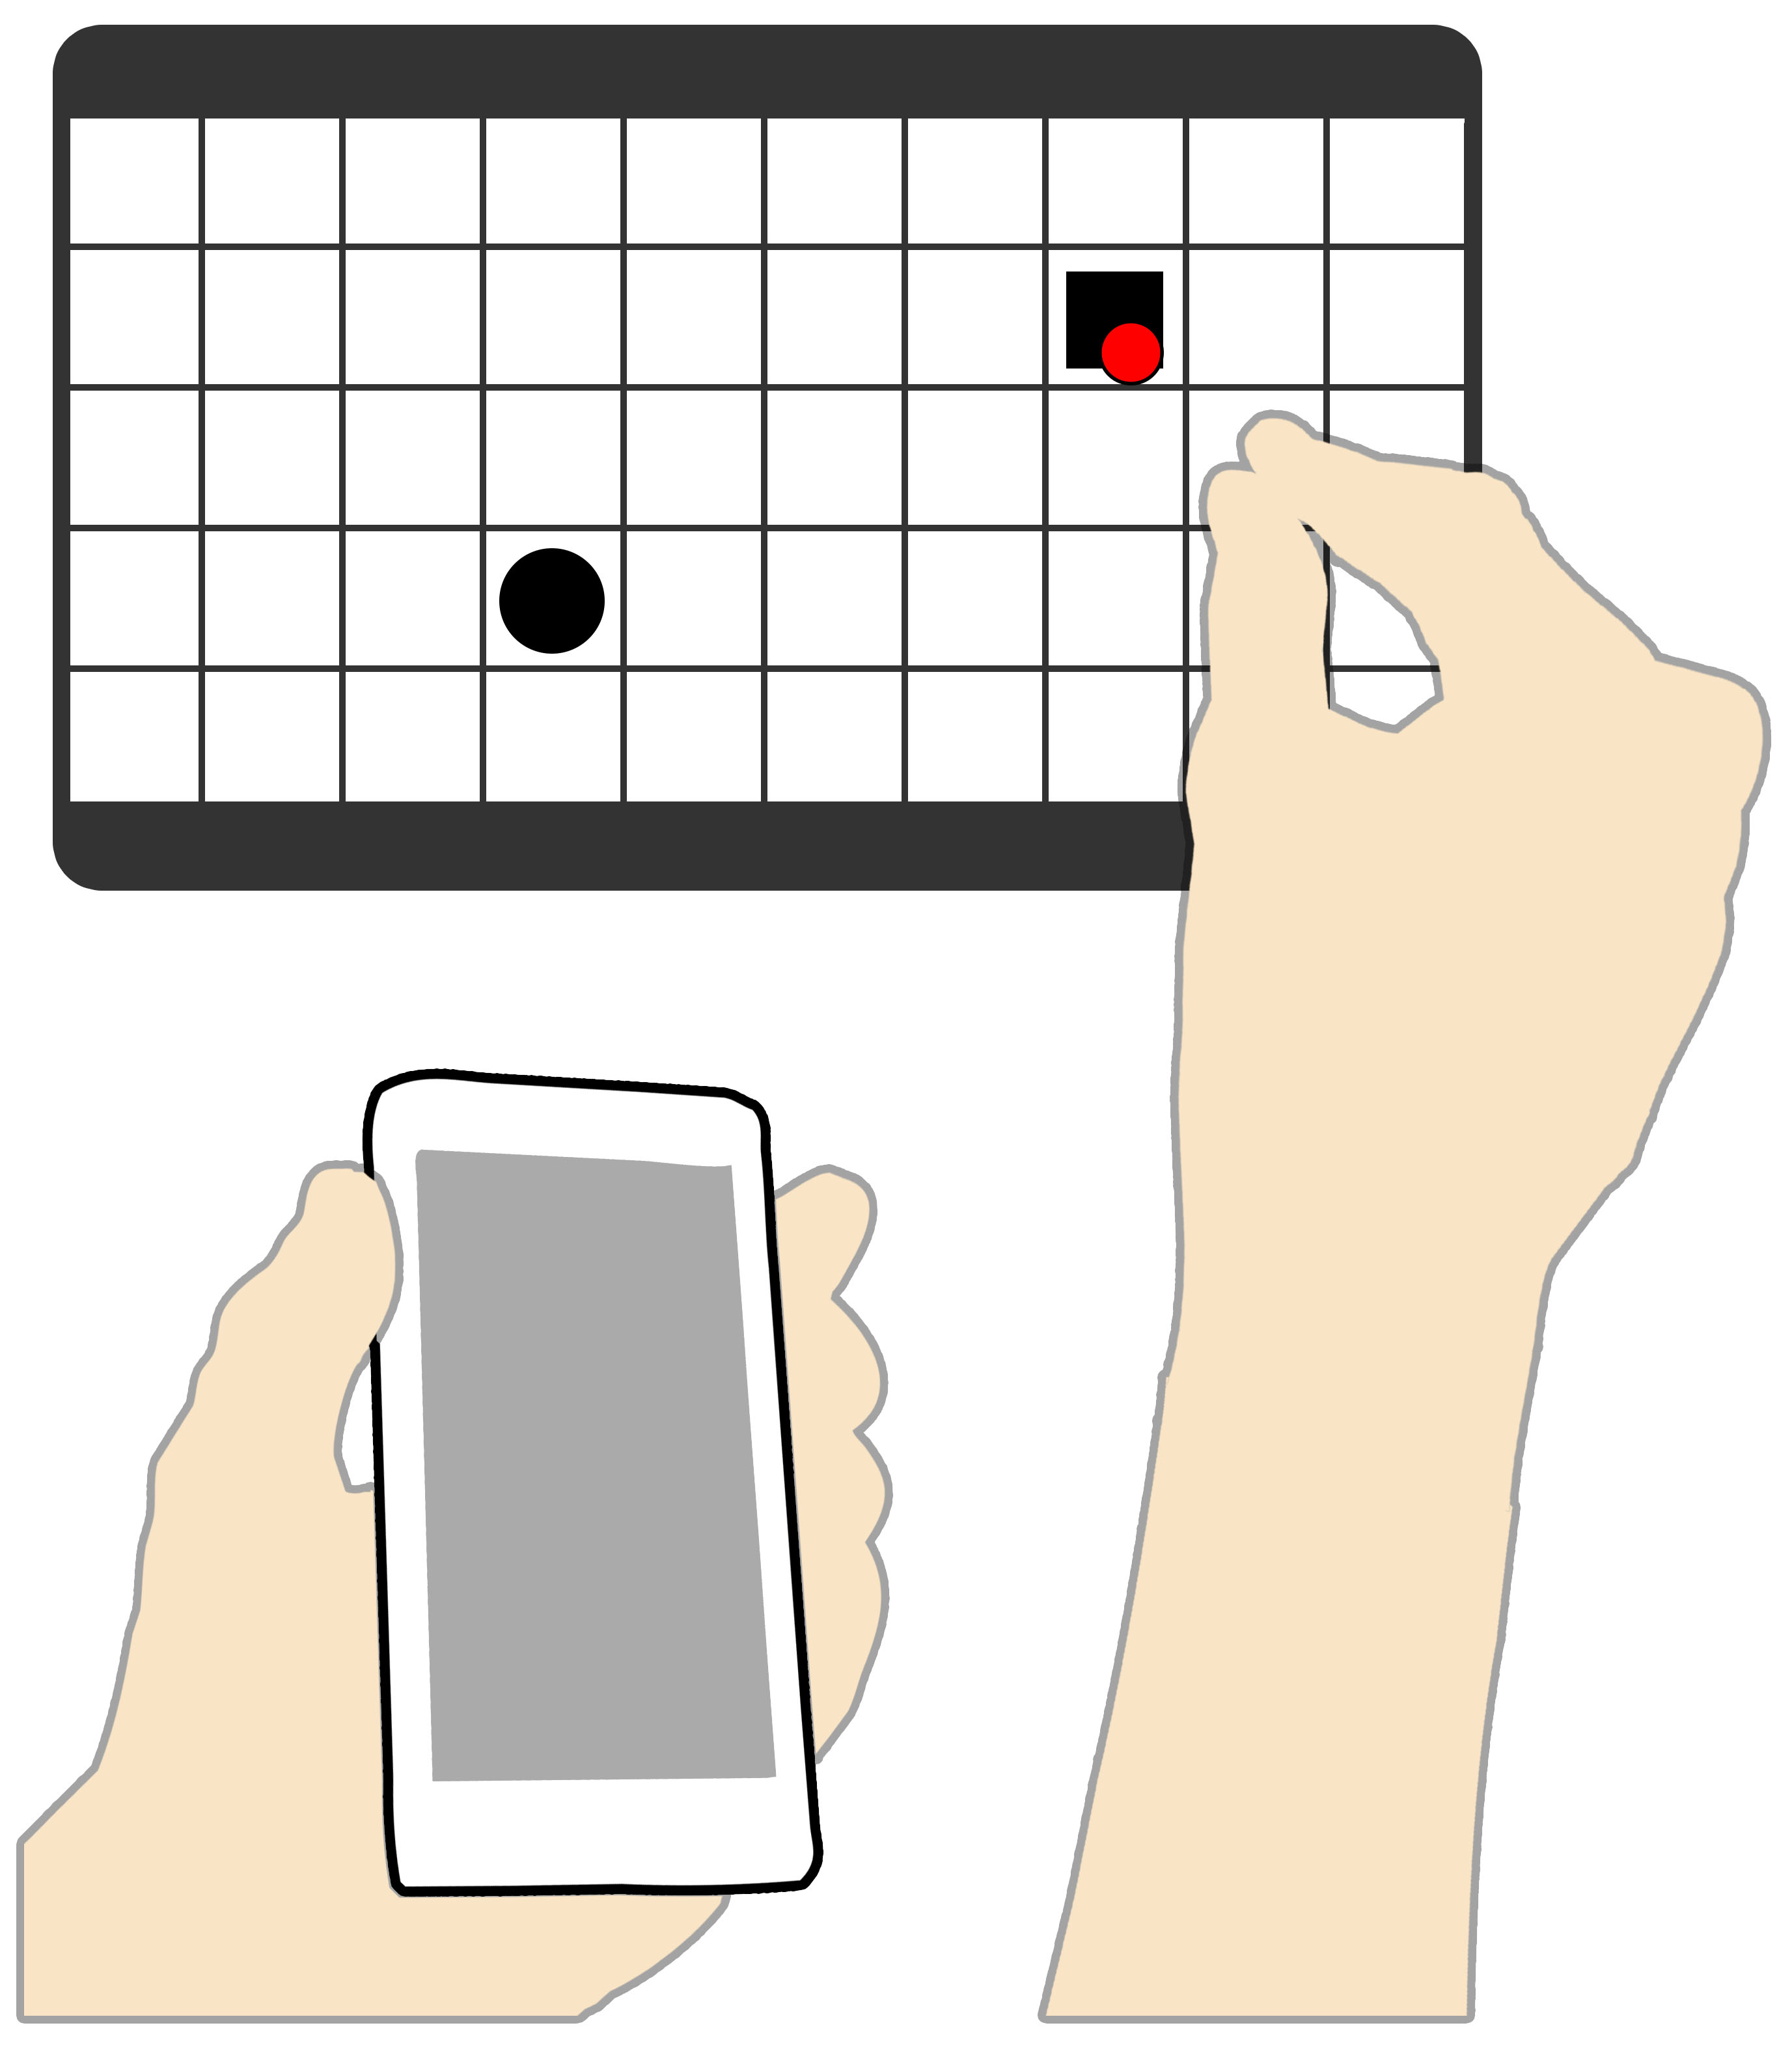
\includegraphics[width = 0.33\columnwidth]{images/techniques/grabPull2.jpg}\label{fig:grabPull2}}
	\subfloat[]{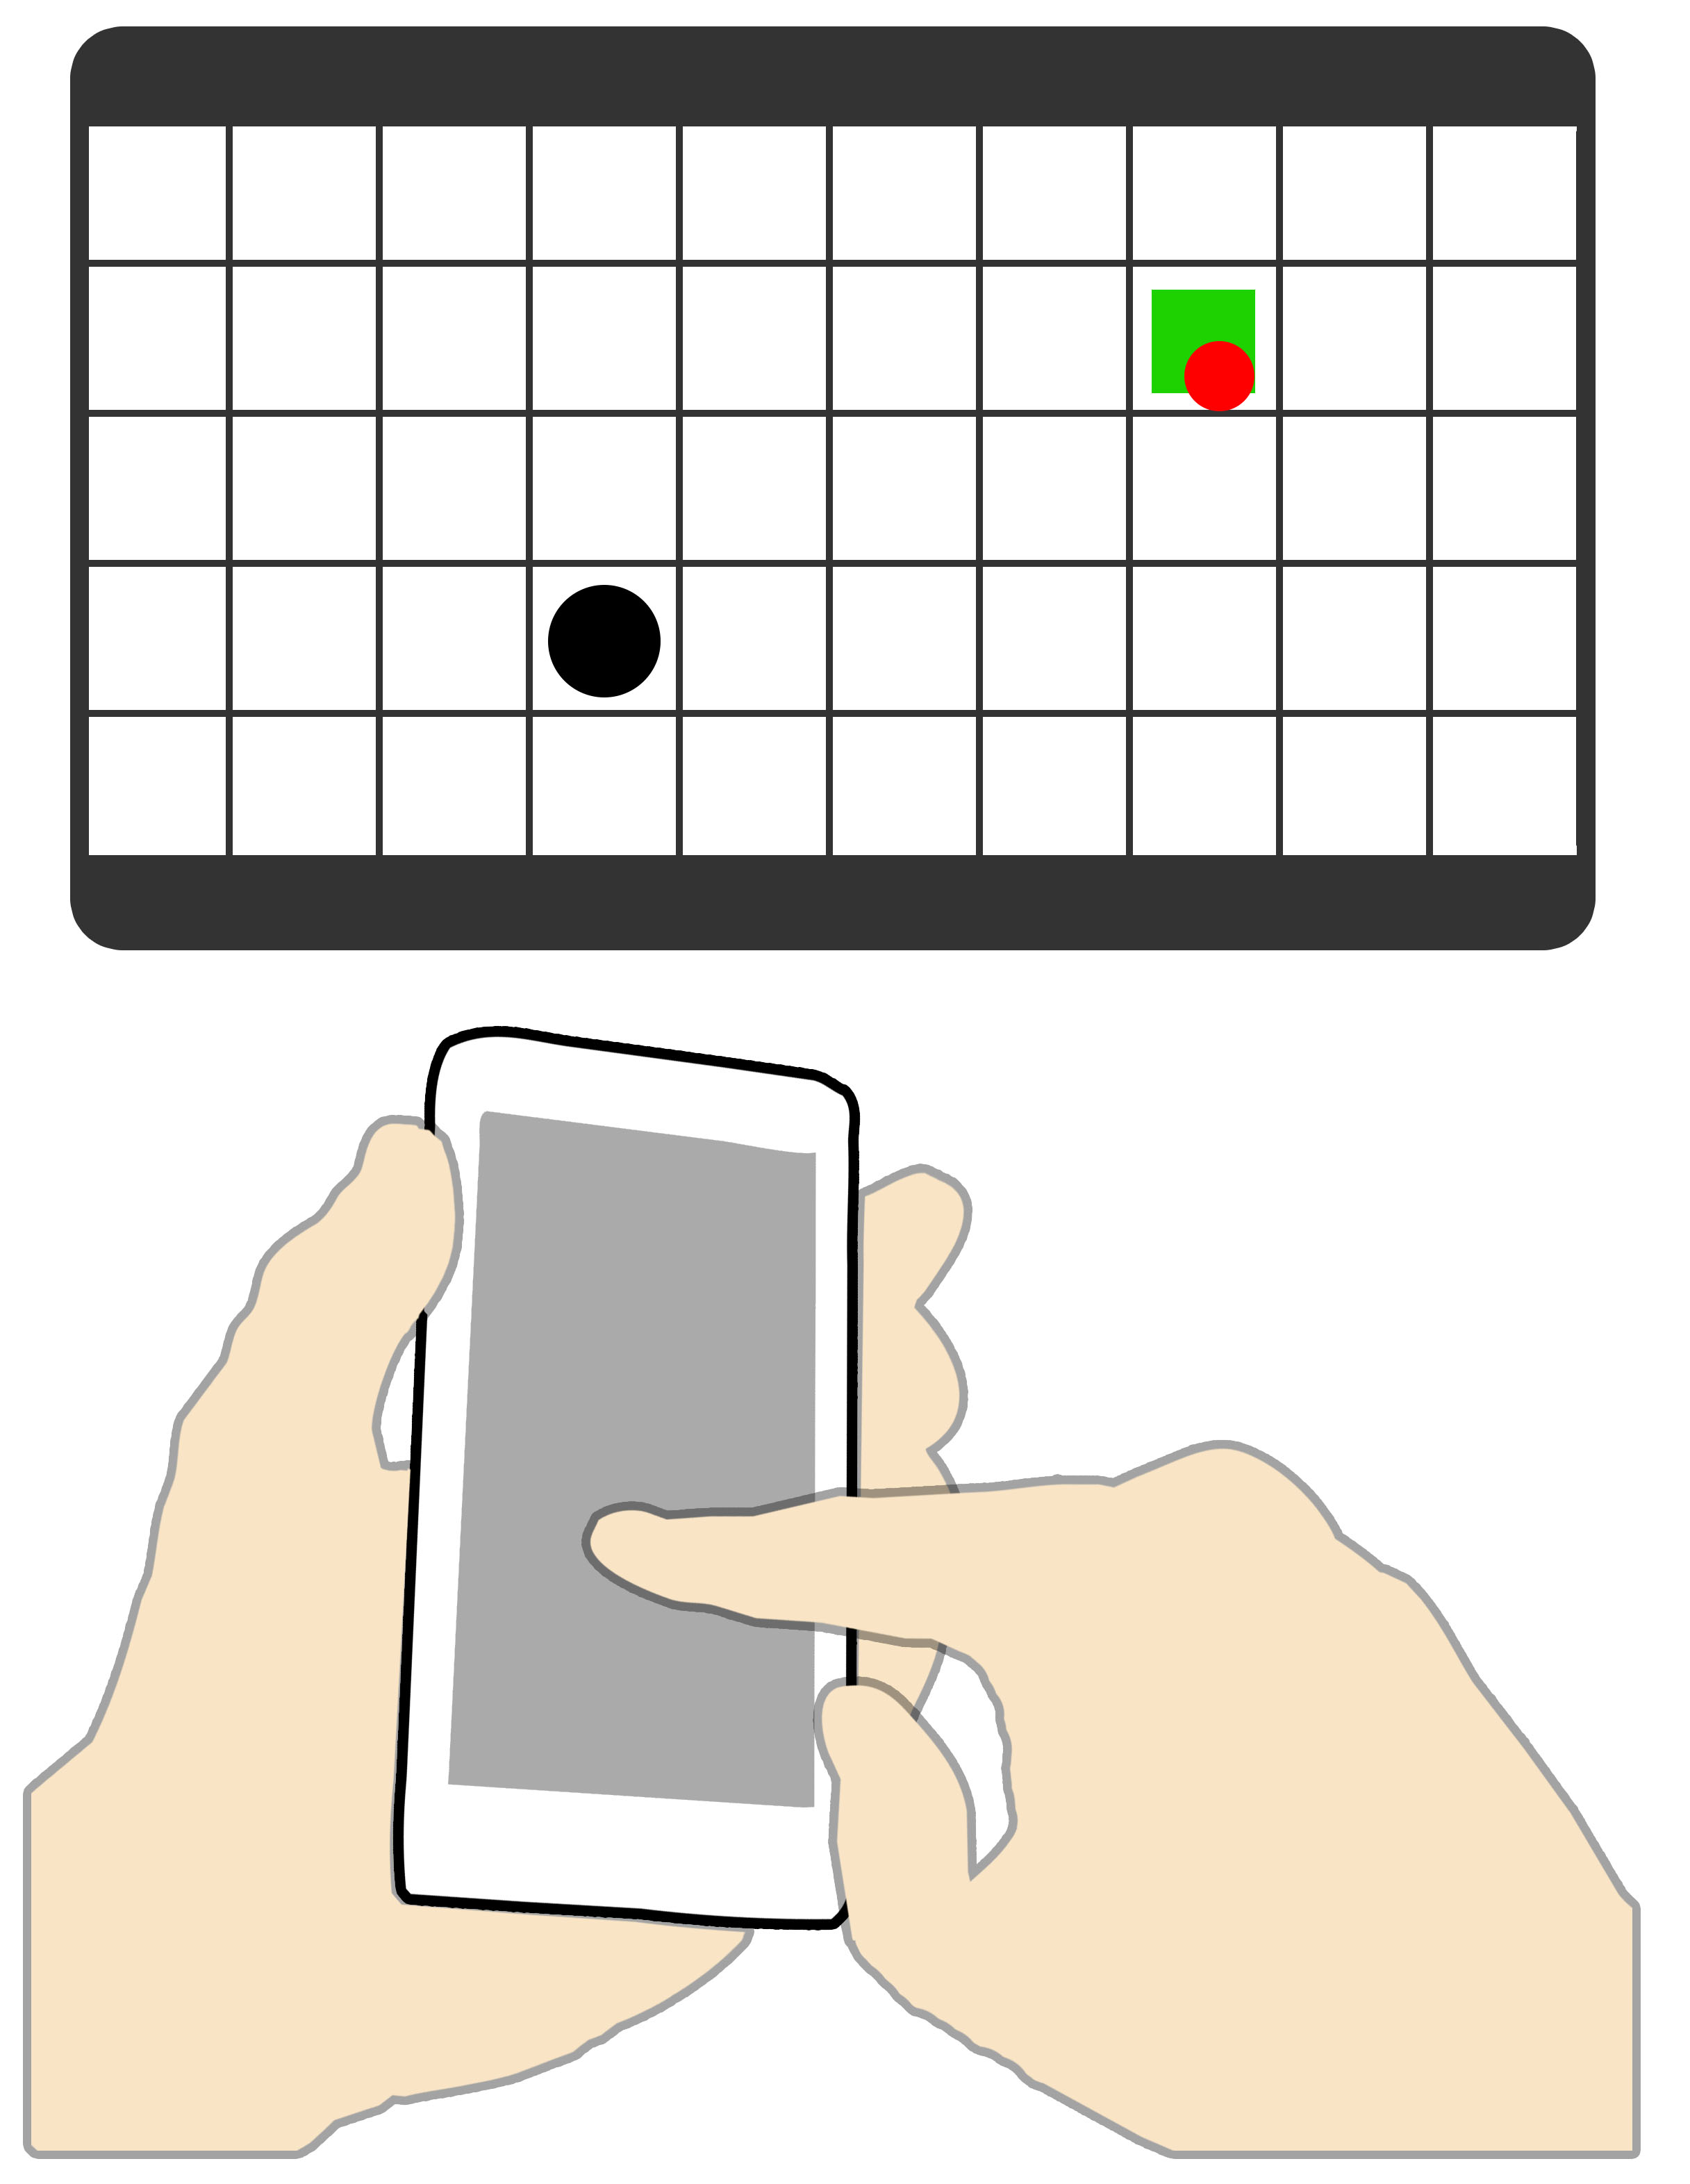
\includegraphics[width = 0.33\columnwidth]{images/techniques/grabPull3.jpg}\label{fig:grabPull3}}
	\caption{\push \grab technique}
	\label{fig:grabTechnique}
\end{figure}

\begin{figure}[H]
	\subfloat[]{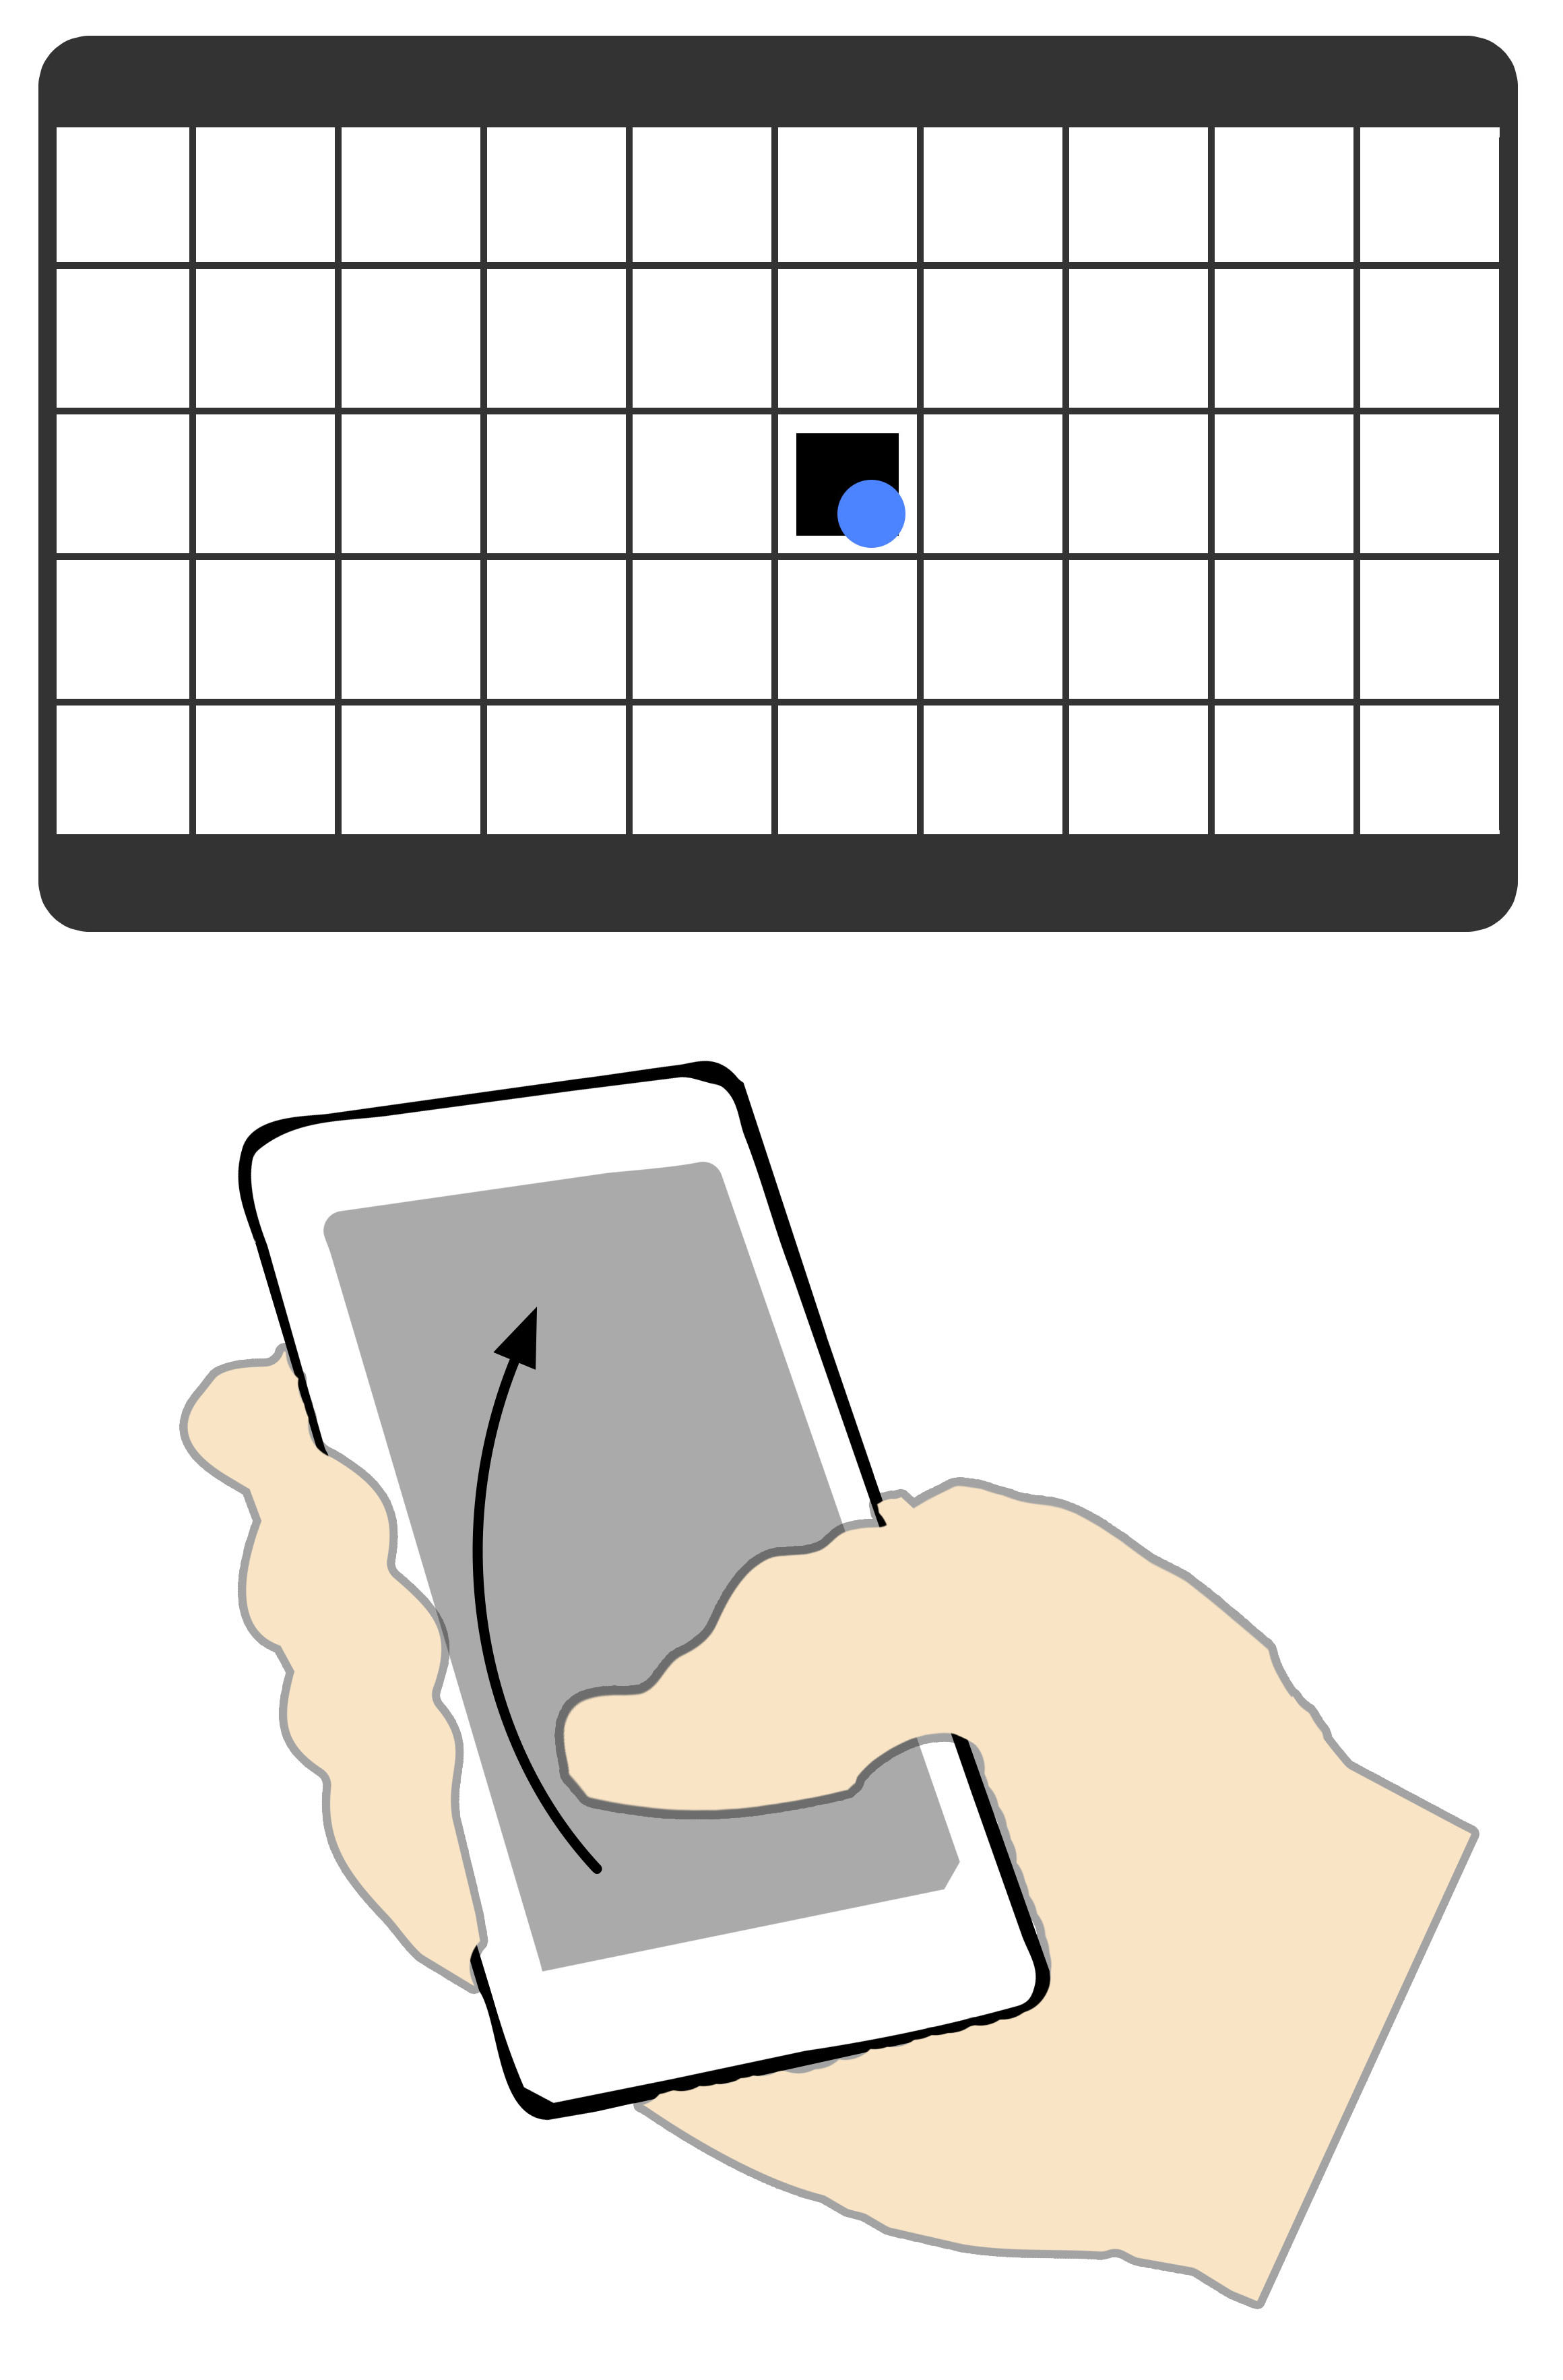
\includegraphics[width = 0.33\columnwidth]{images/techniques/swipePush1.jpg}\label{fig:swipePush1}}
	\subfloat[]{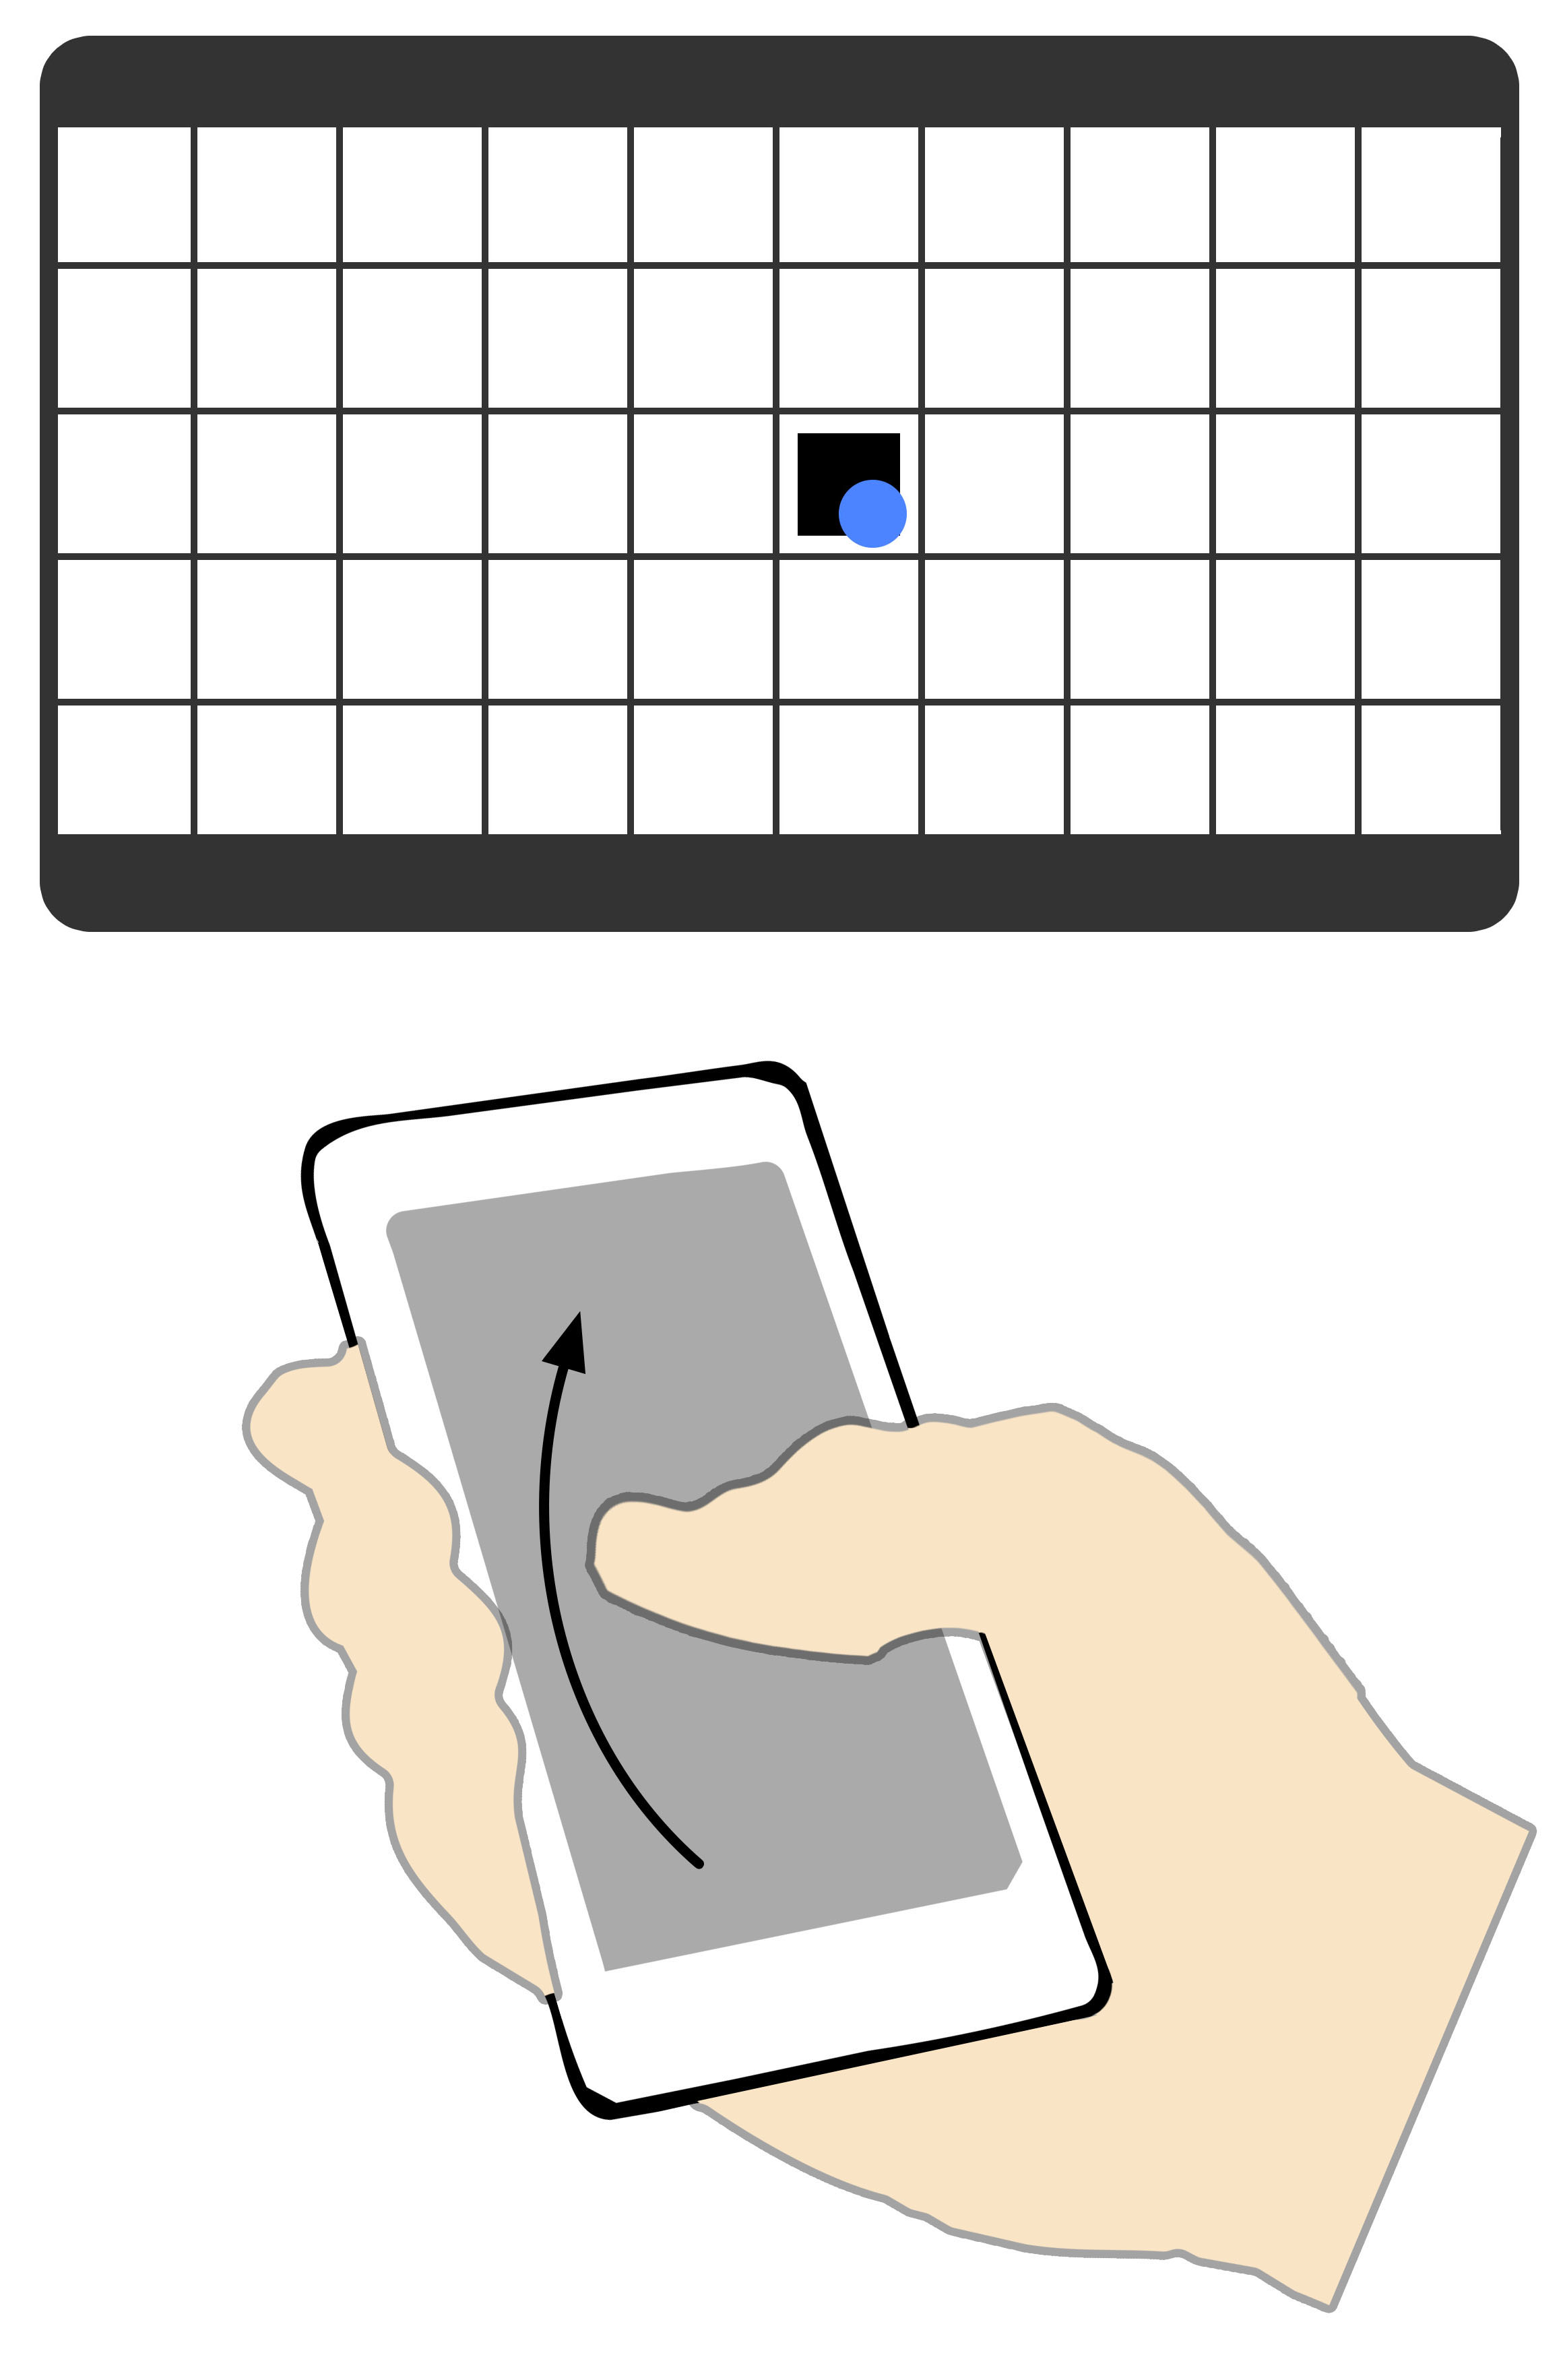
\includegraphics[width = 0.33\columnwidth]{images/techniques/swipePush2.jpg}\label{fig:swipePush2}}
	\subfloat[]{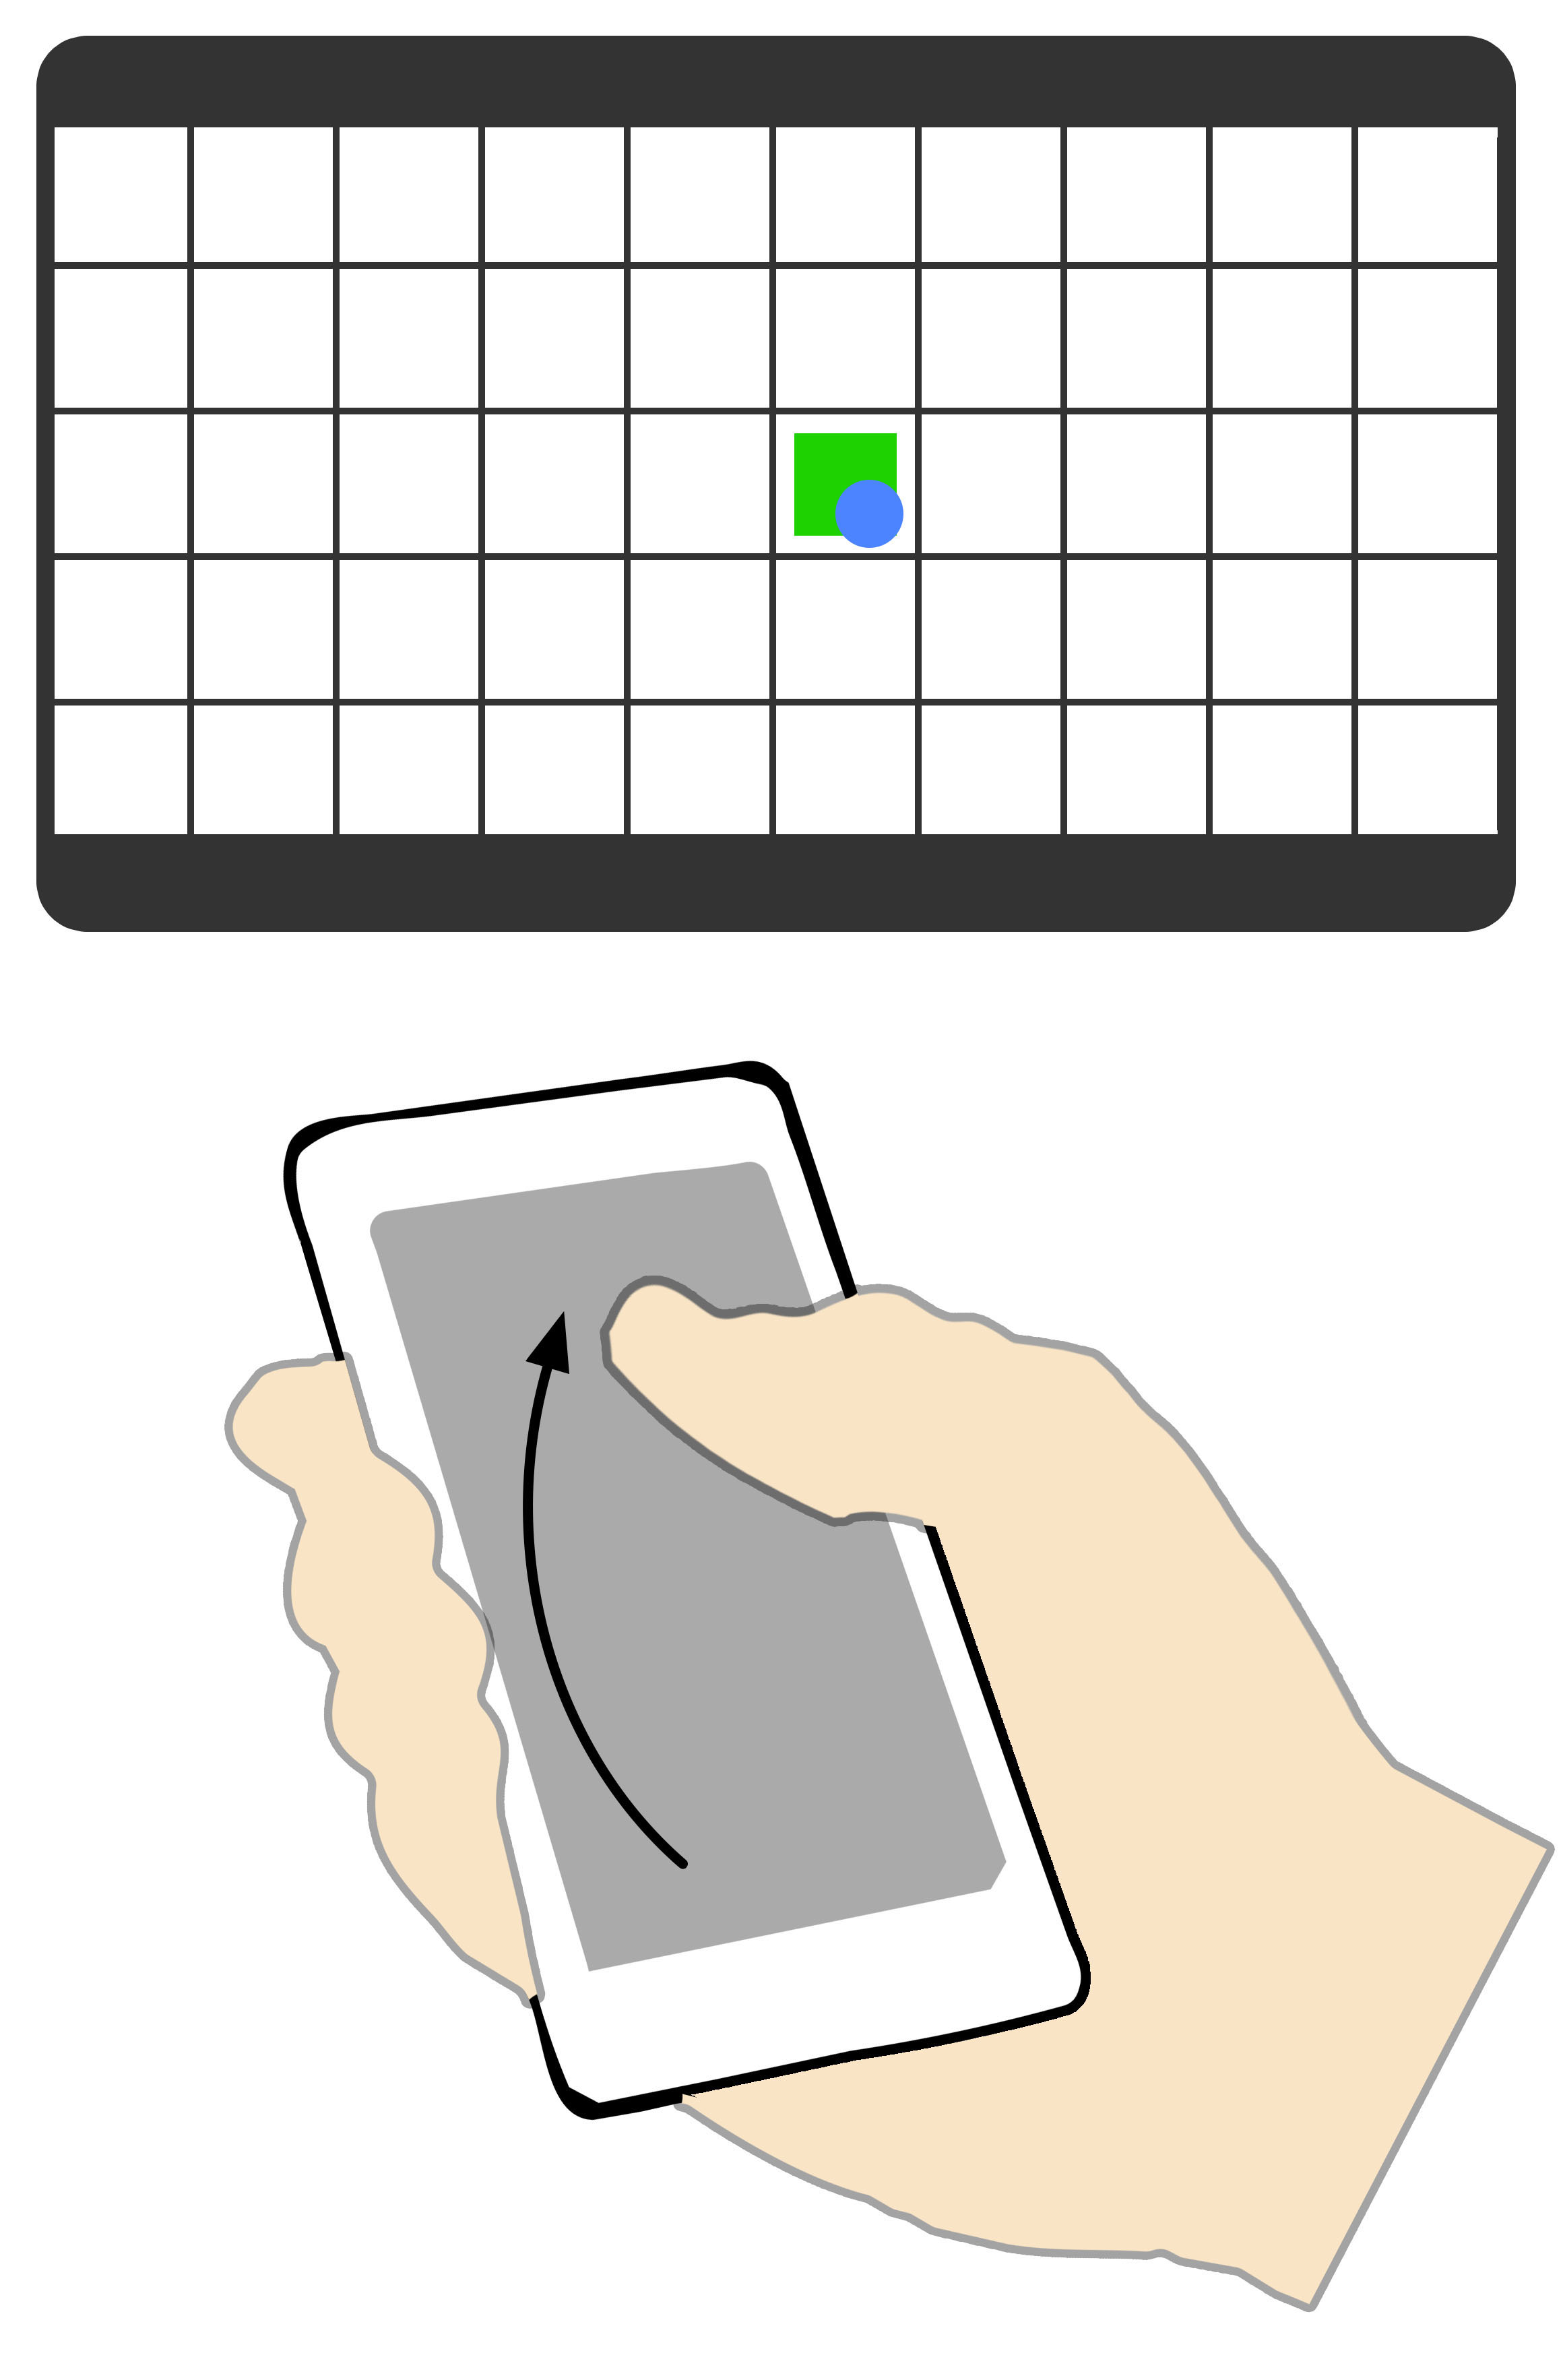
\includegraphics[width = 0.33\columnwidth]{images/techniques/swipePush3.jpg}\label{fig:swipePush3}}
	\caption{\push \grab technique}
	\label{fig:grabTechnique}
\end{figure}

\begin{figure}[H]
	\subfloat[]{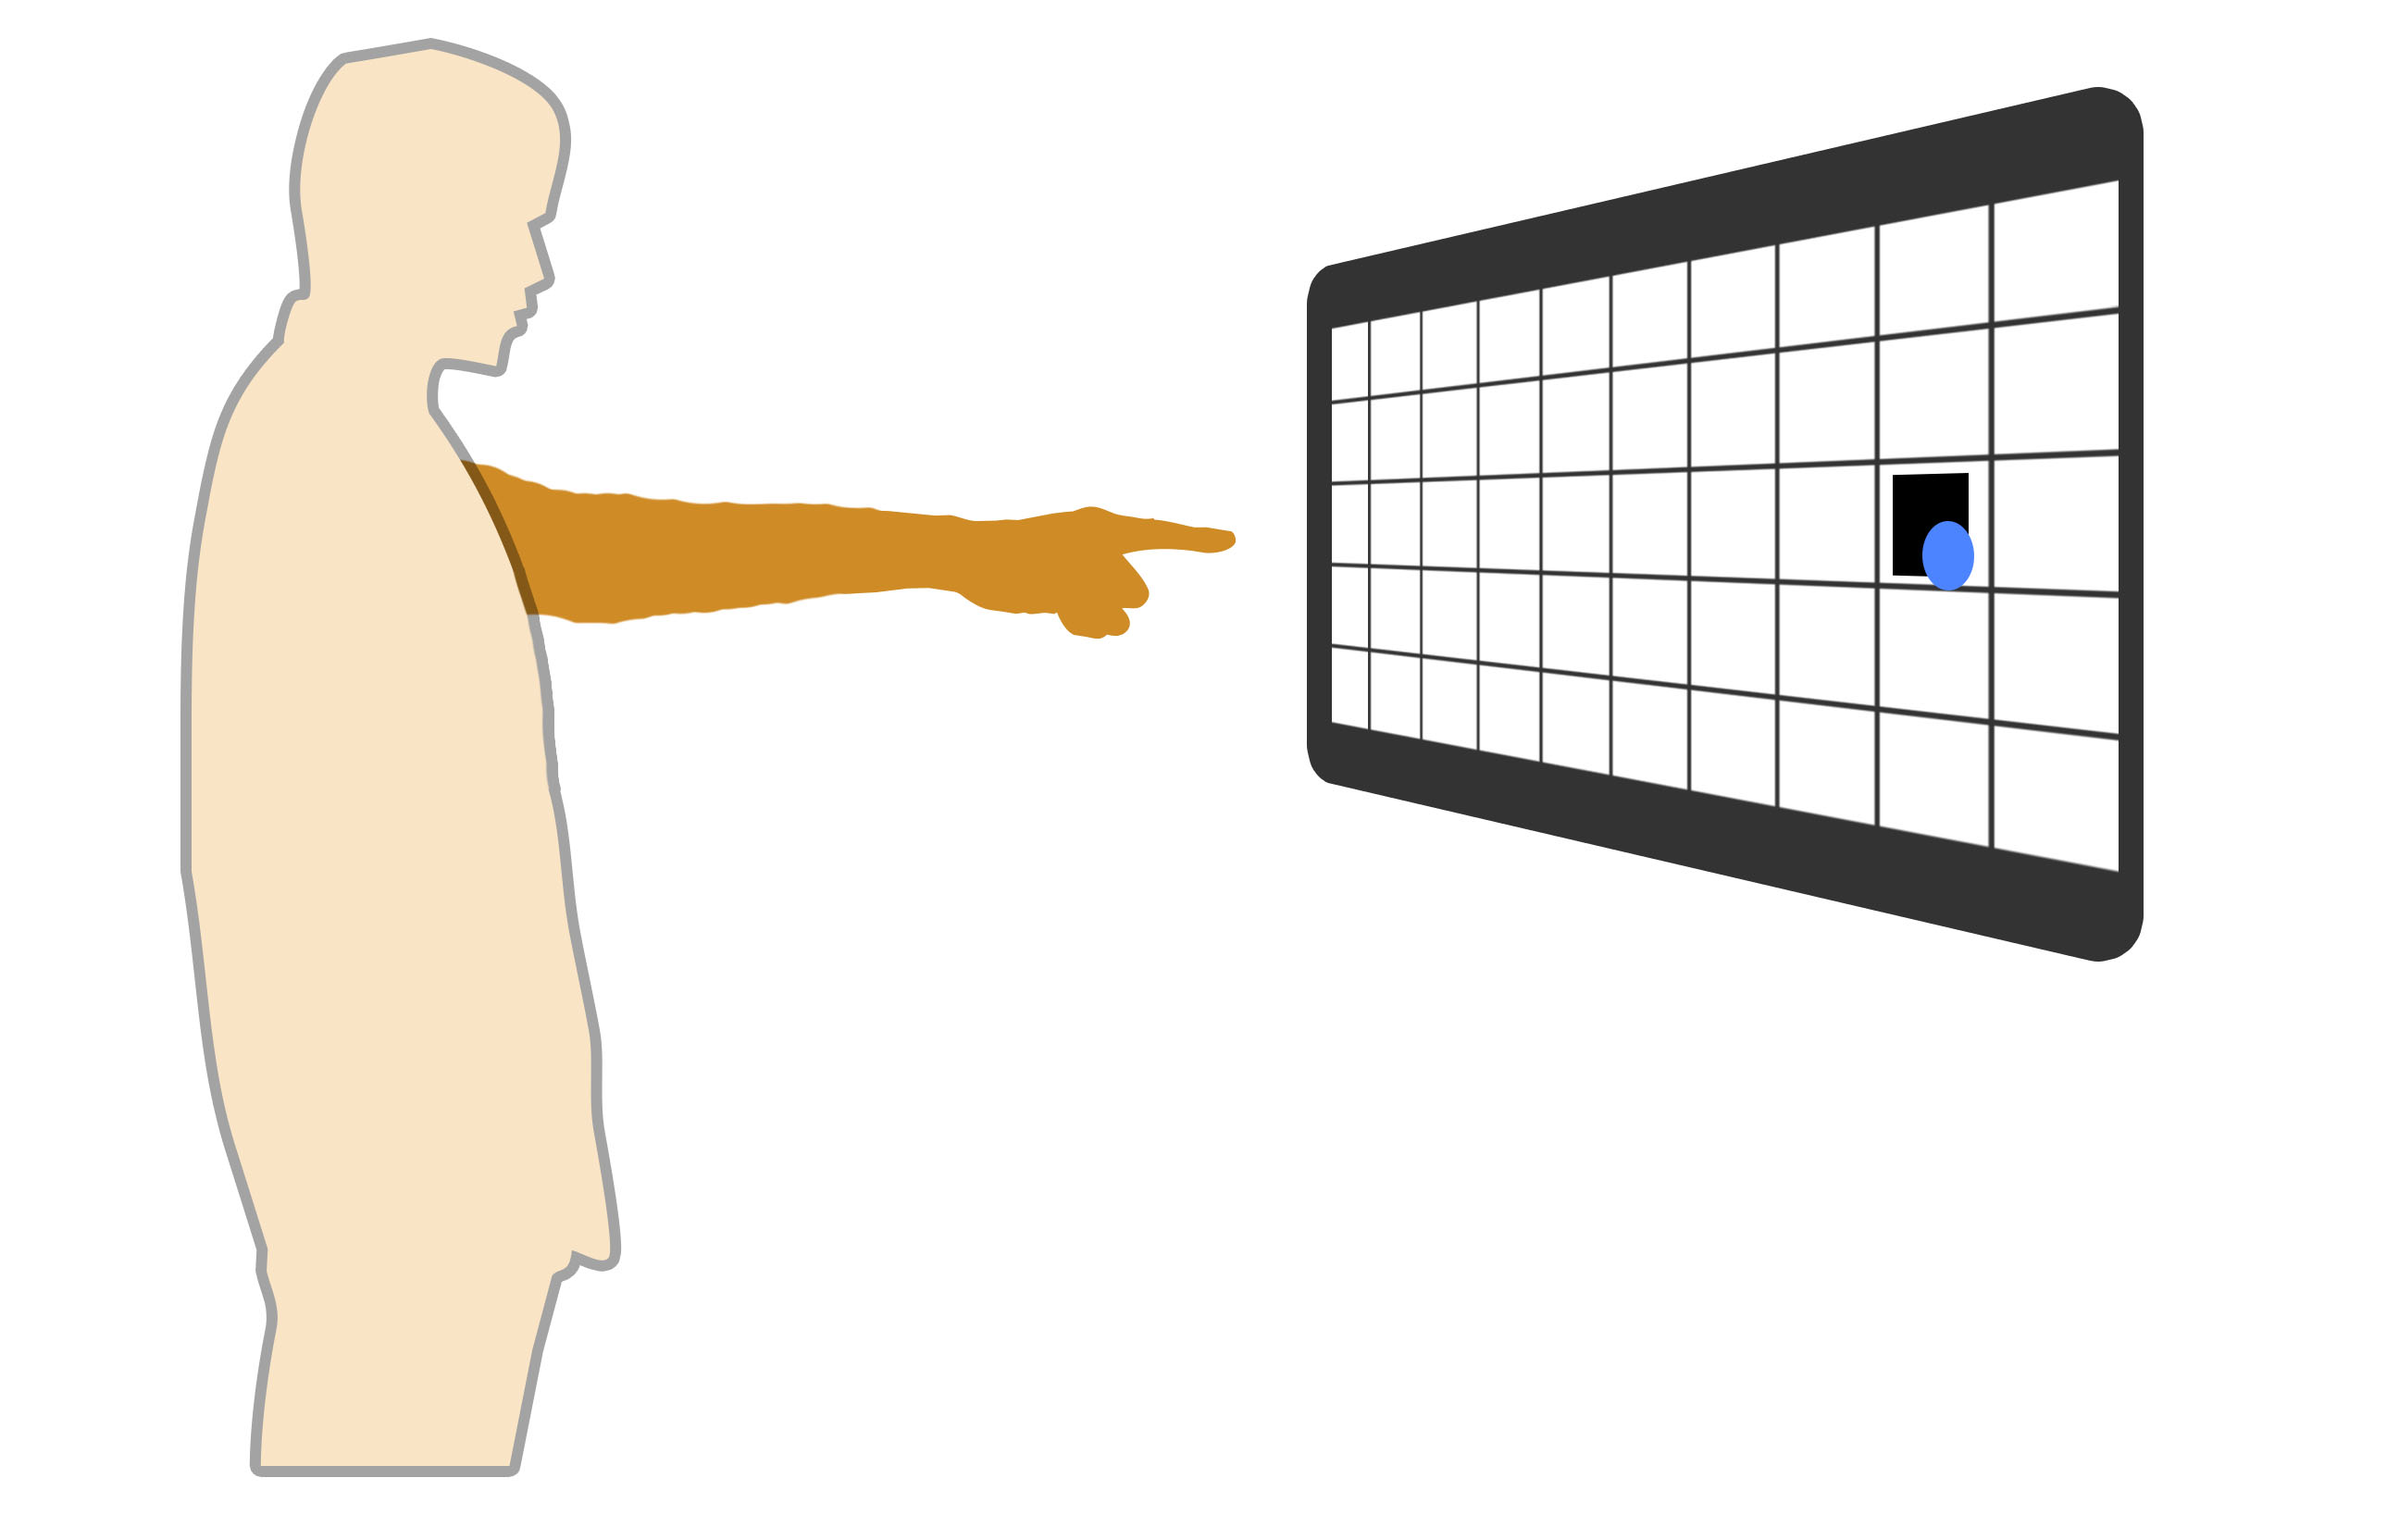
\includegraphics[width = 0.33\columnwidth]{images/techniques/throwPush1.jpg}\label{fig:throwPush1}}
	\subfloat[]{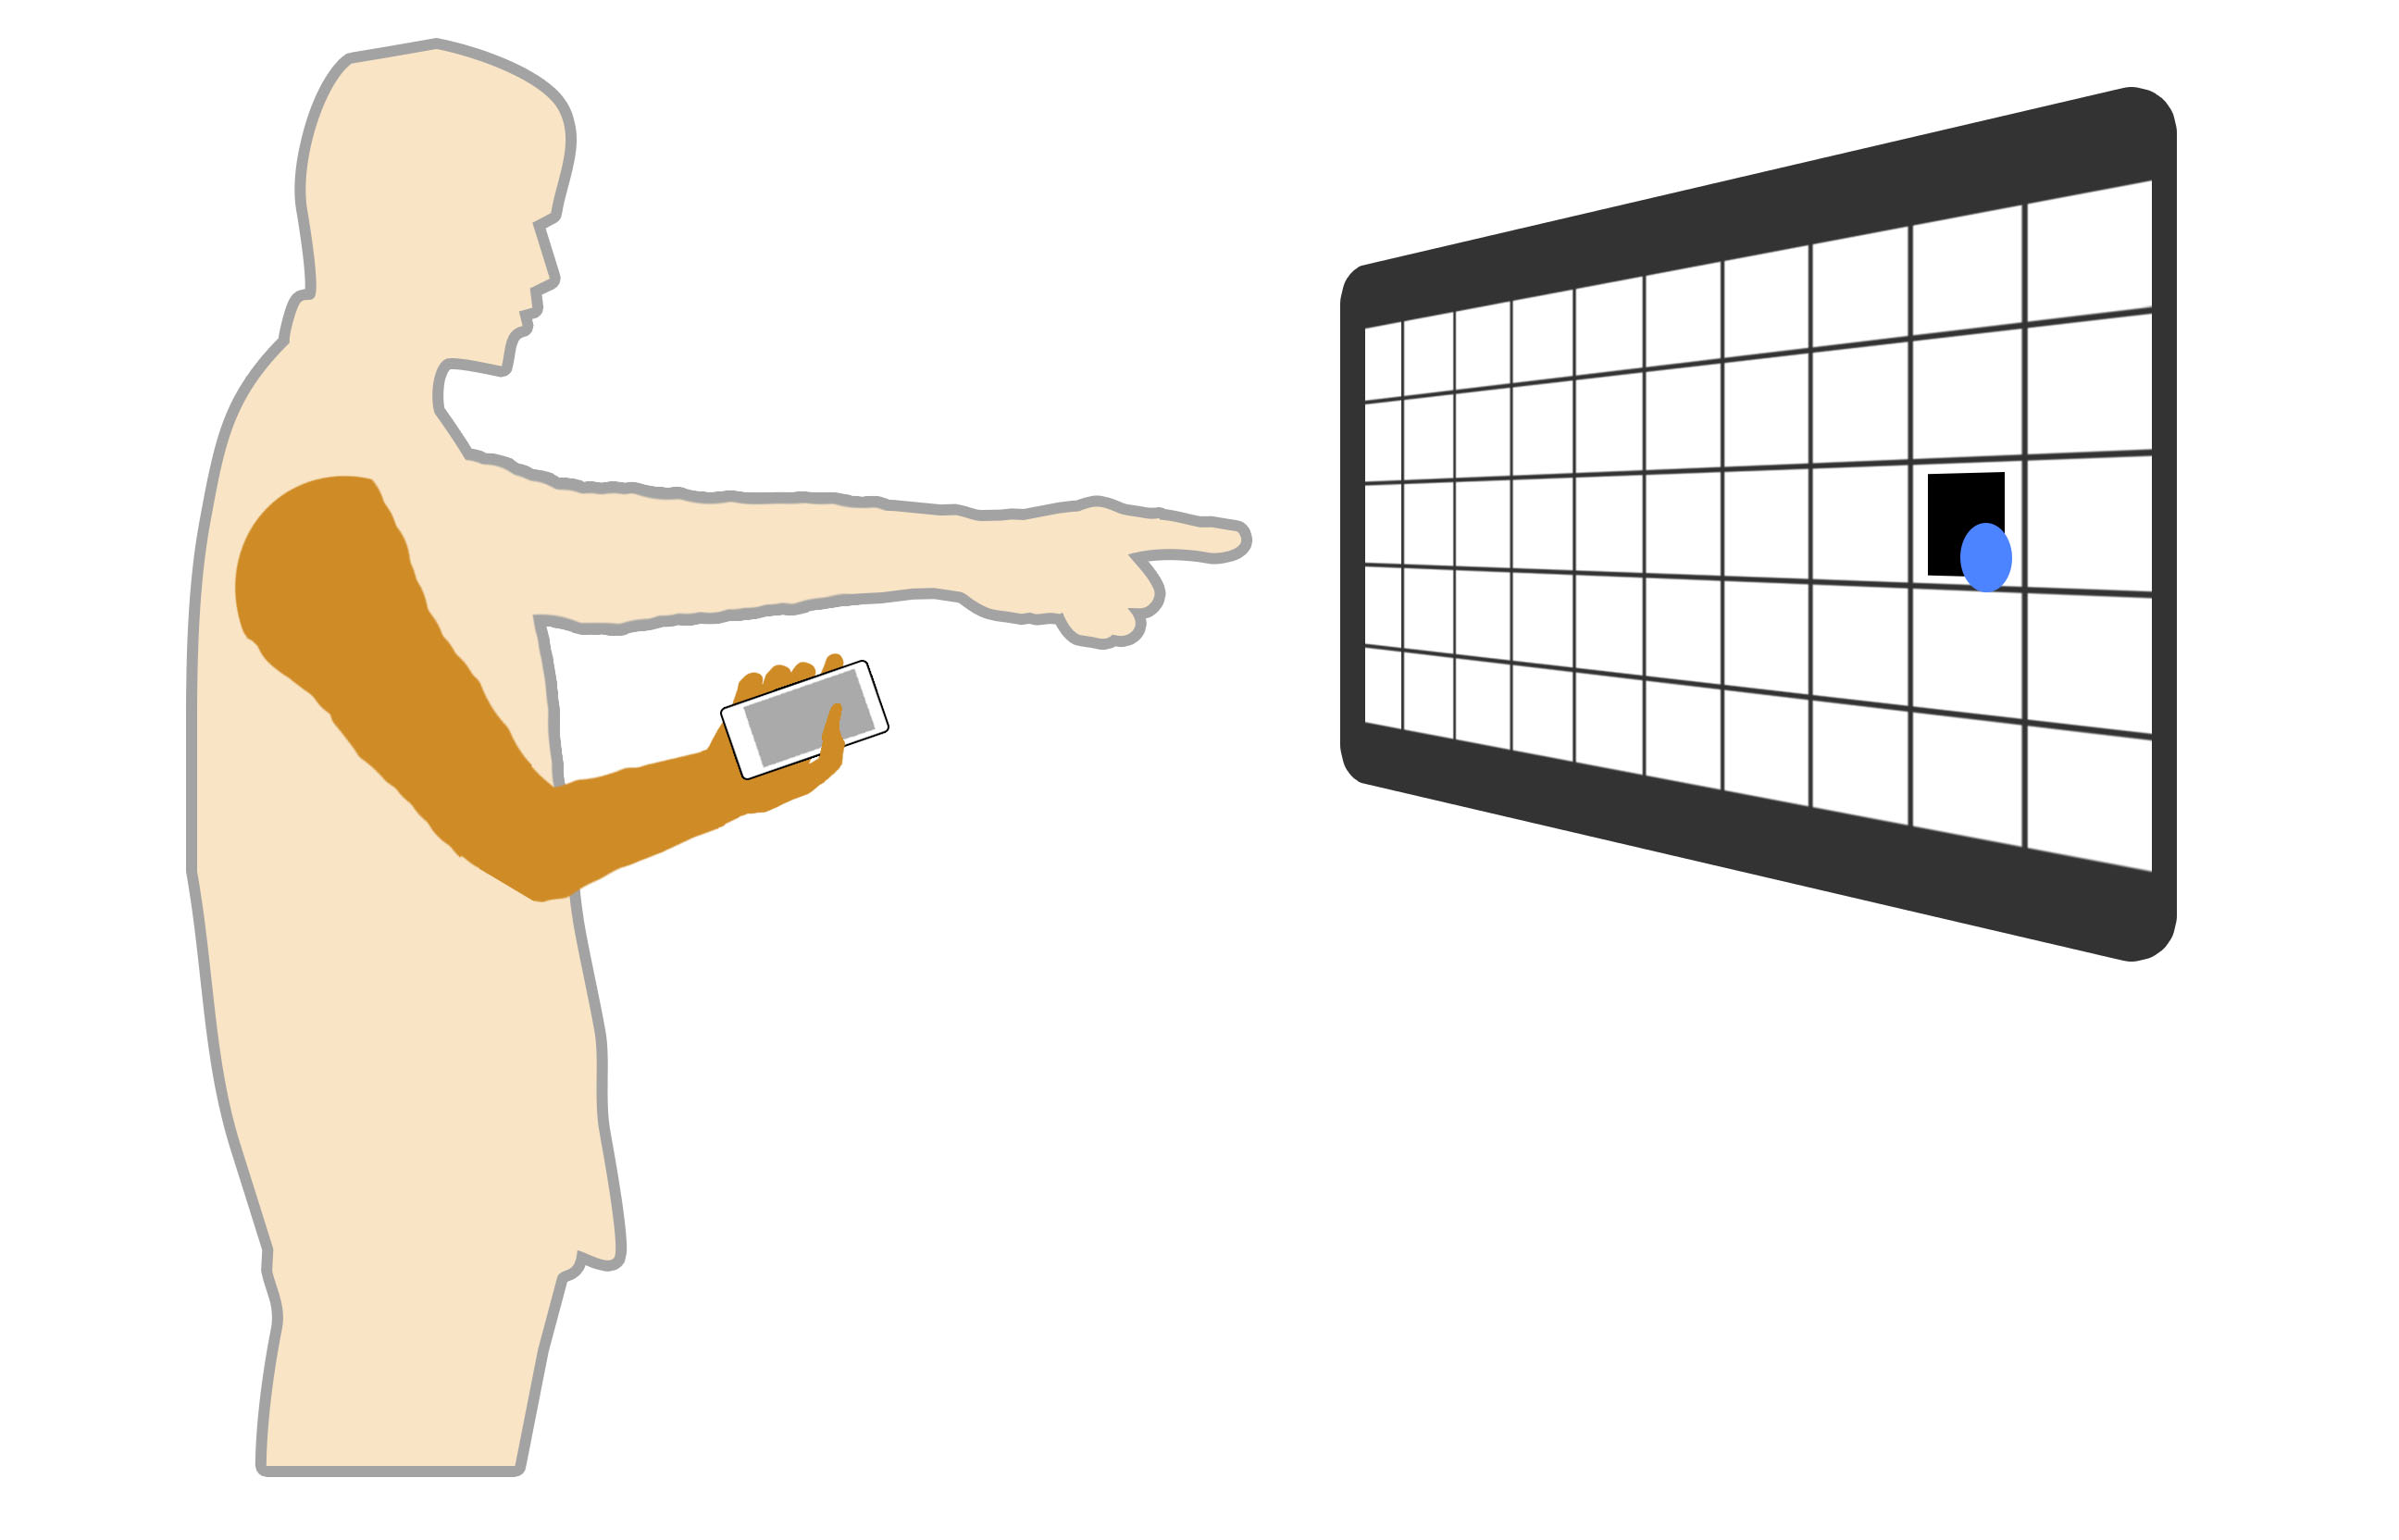
\includegraphics[width = 0.33\columnwidth]{images/techniques/throwPush2.jpg}\label{fig:throwPush2}}
	\subfloat[]{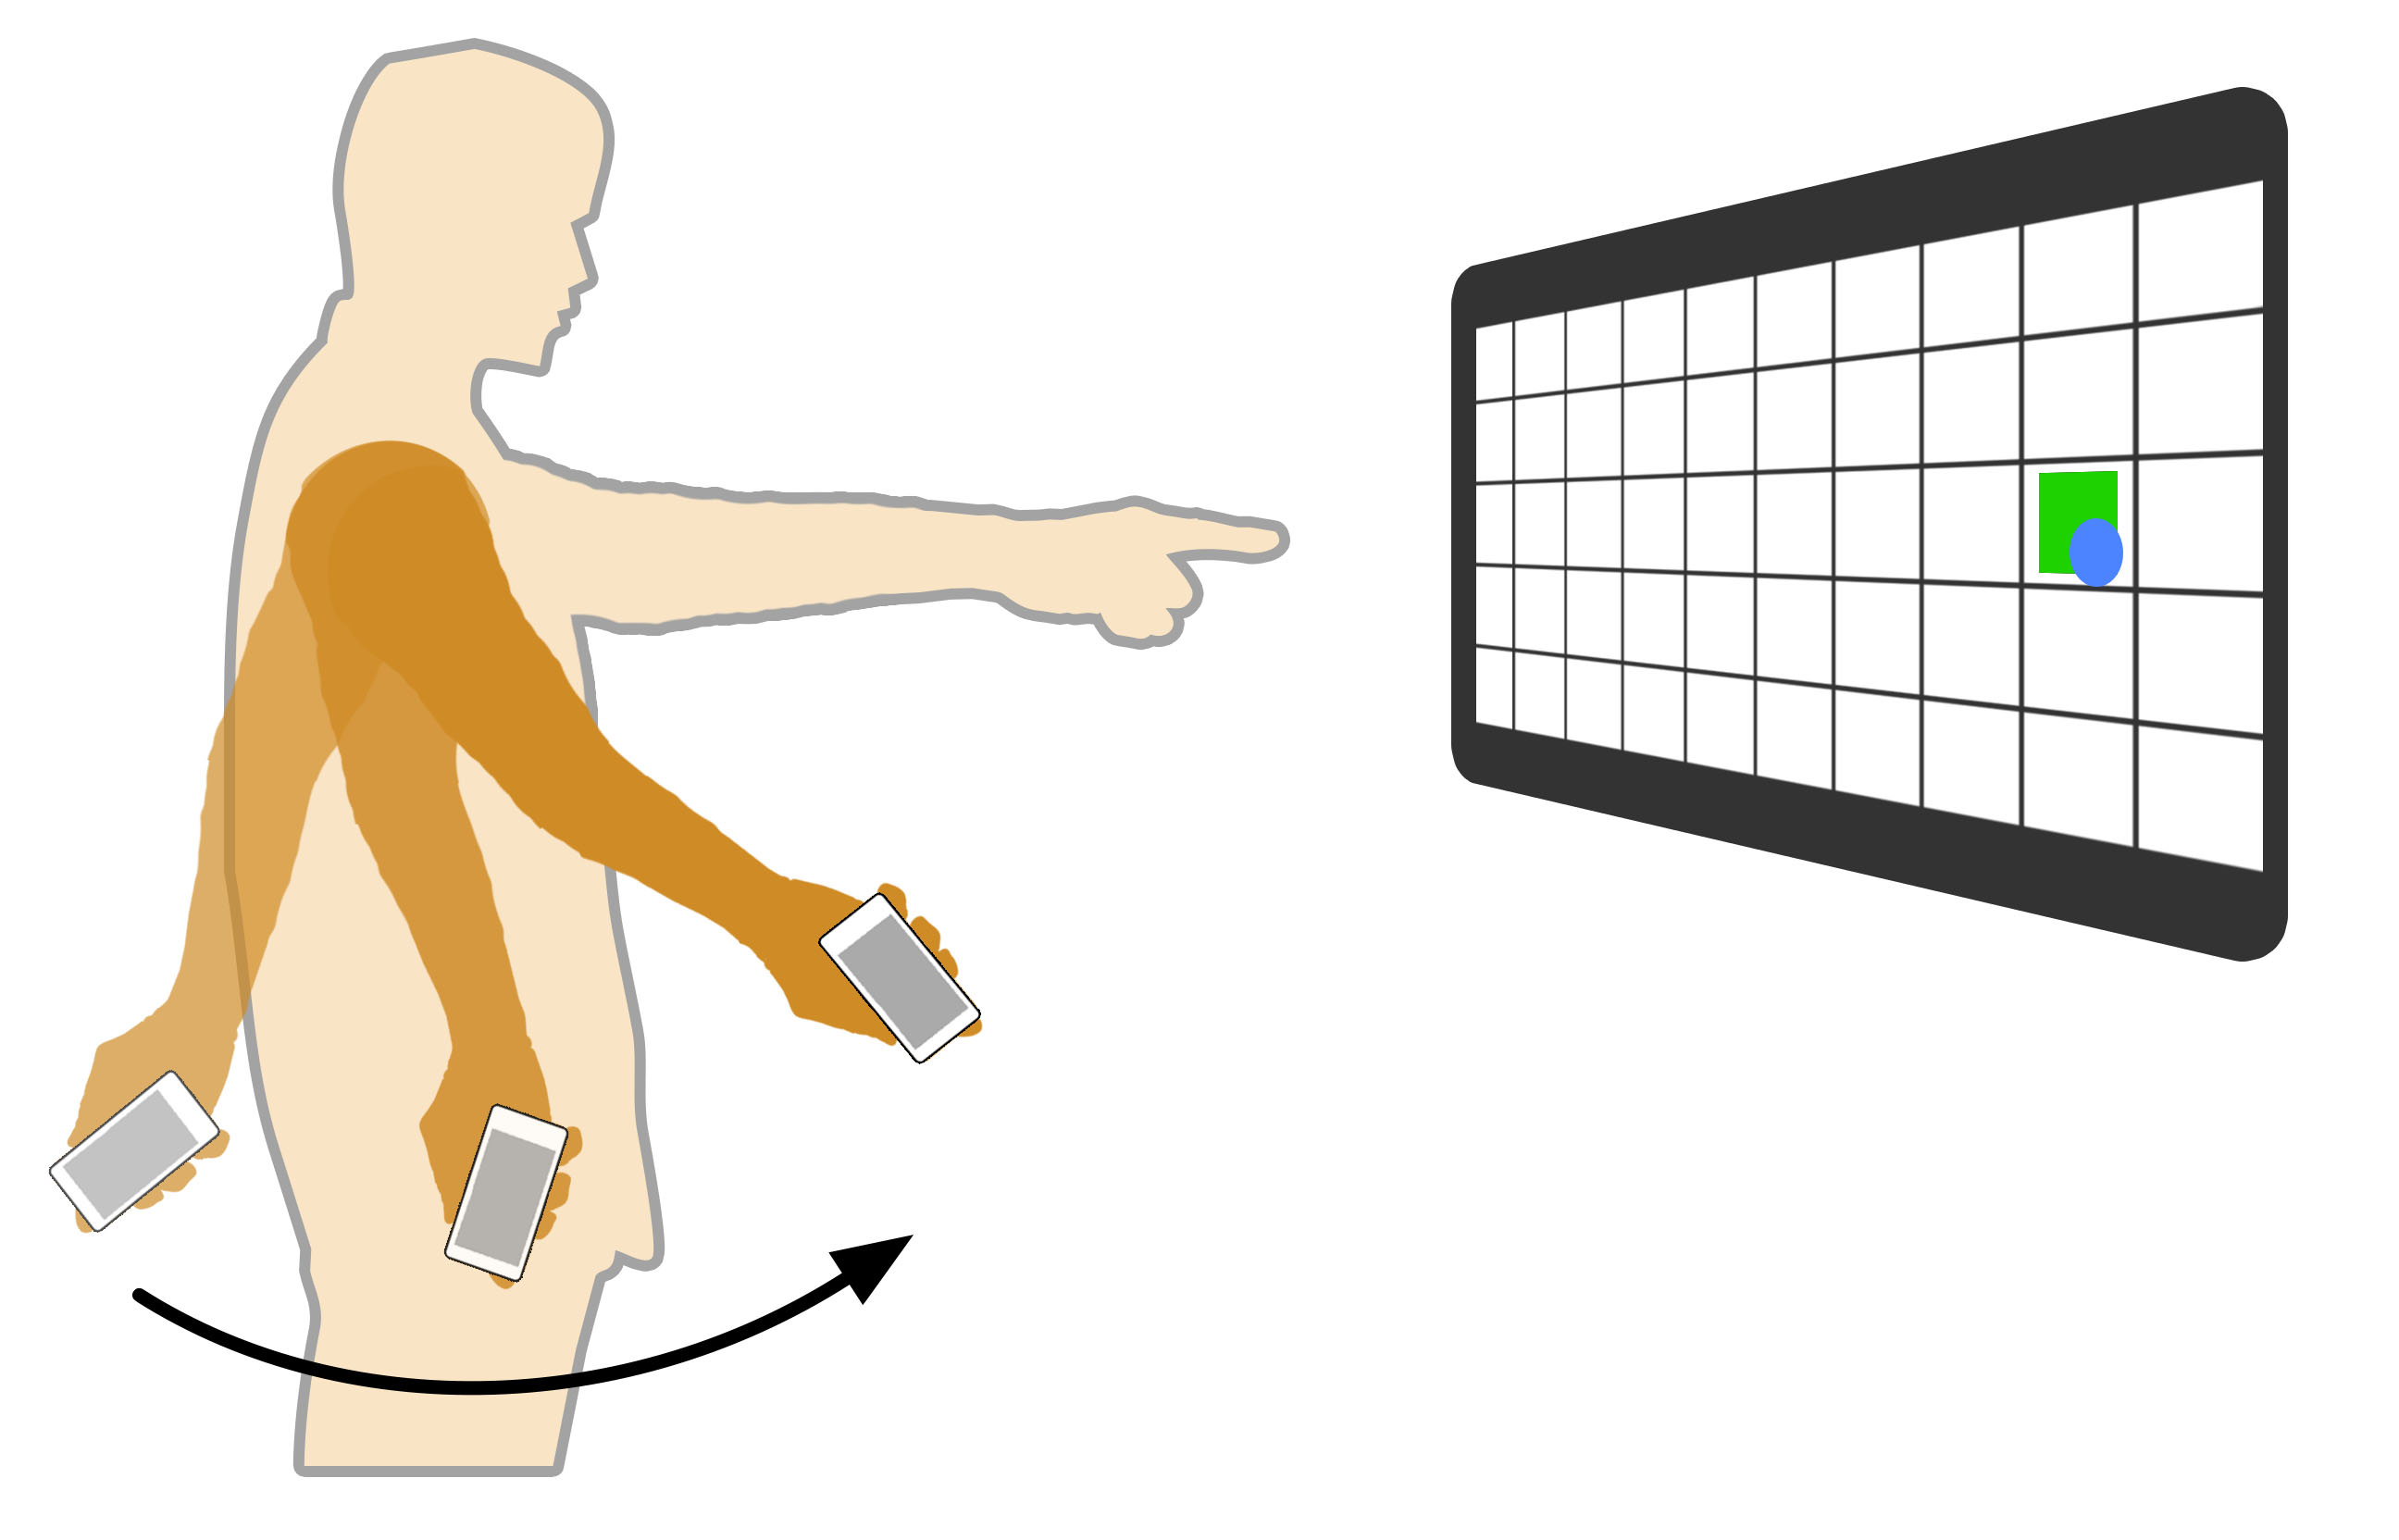
\includegraphics[width = 0.33\columnwidth]{images/techniques/throwPush3.jpg}\label{fig:throwPush3}}
	\caption{\push \grab technique}
	\label{fig:grabTechnique}
\end{figure}

\begin{figure}[H]
	\subfloat[]{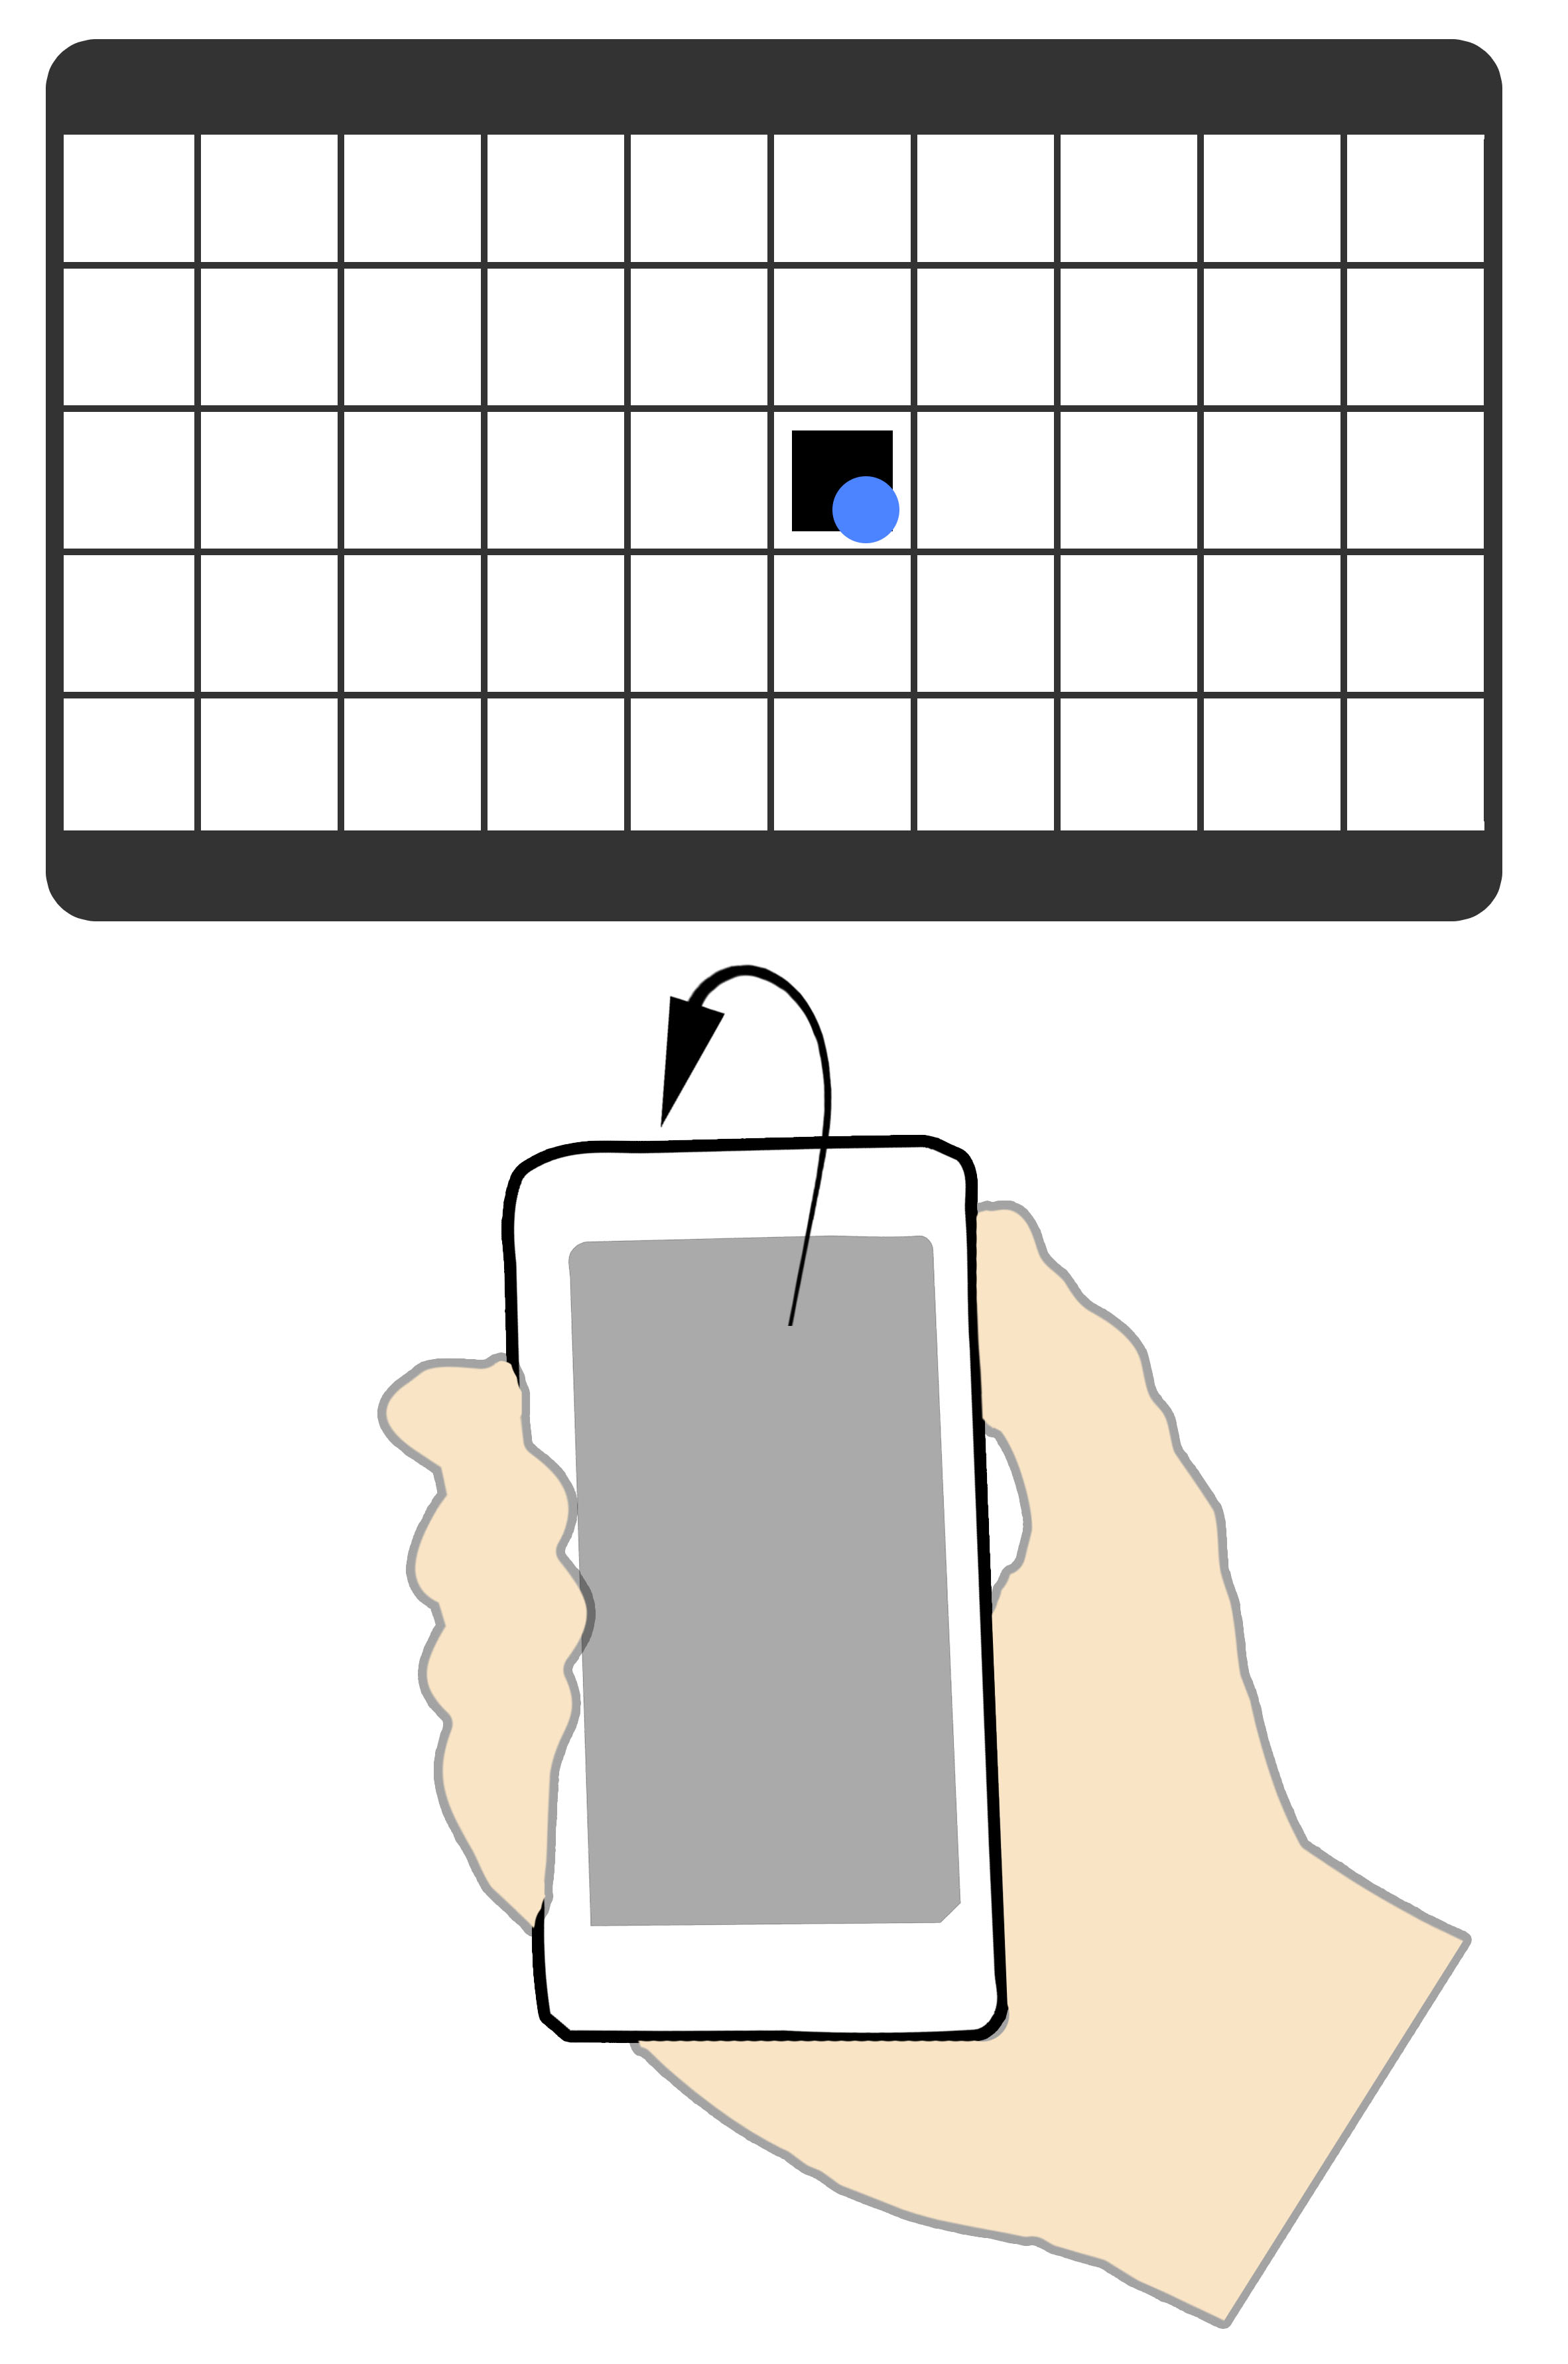
\includegraphics[width = 0.33\columnwidth]{images/techniques/tiltPush1.jpg}\label{fig:tiltPush1}}
	\subfloat[]{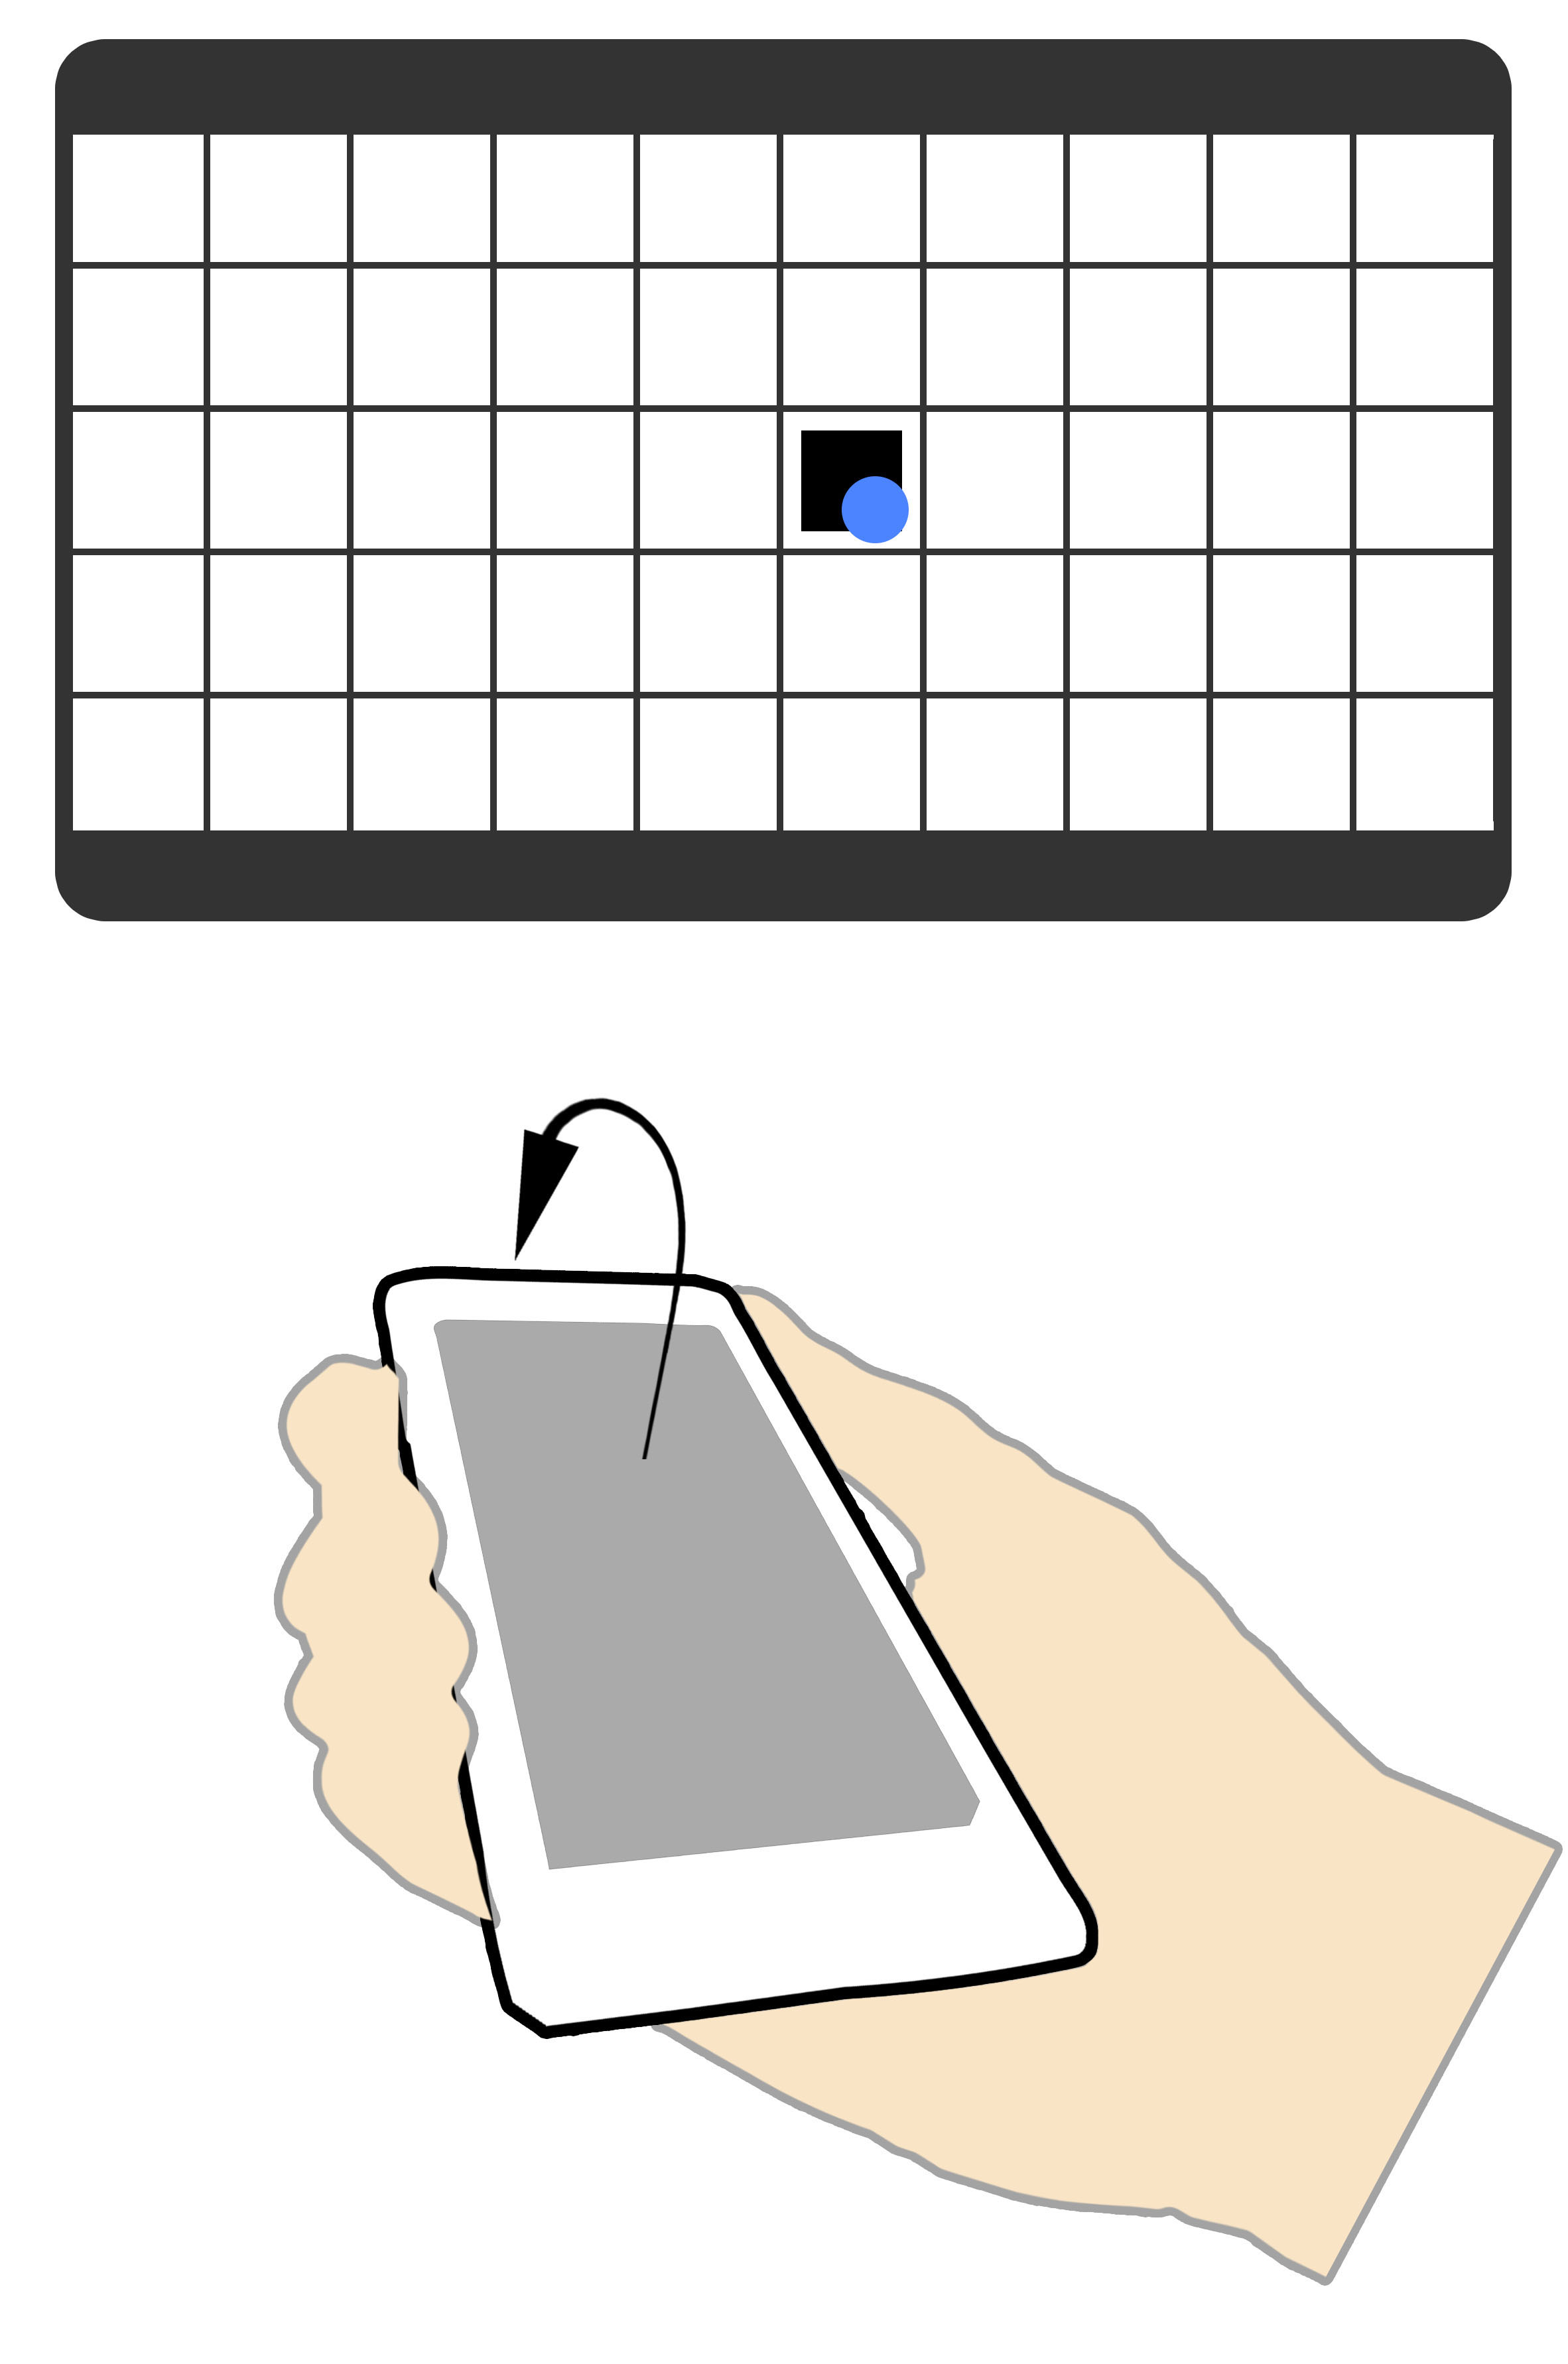
\includegraphics[width = 0.33\columnwidth]{images/techniques/tiltPush2.jpg}\label{fig:tiltPush2}}
	\subfloat[]{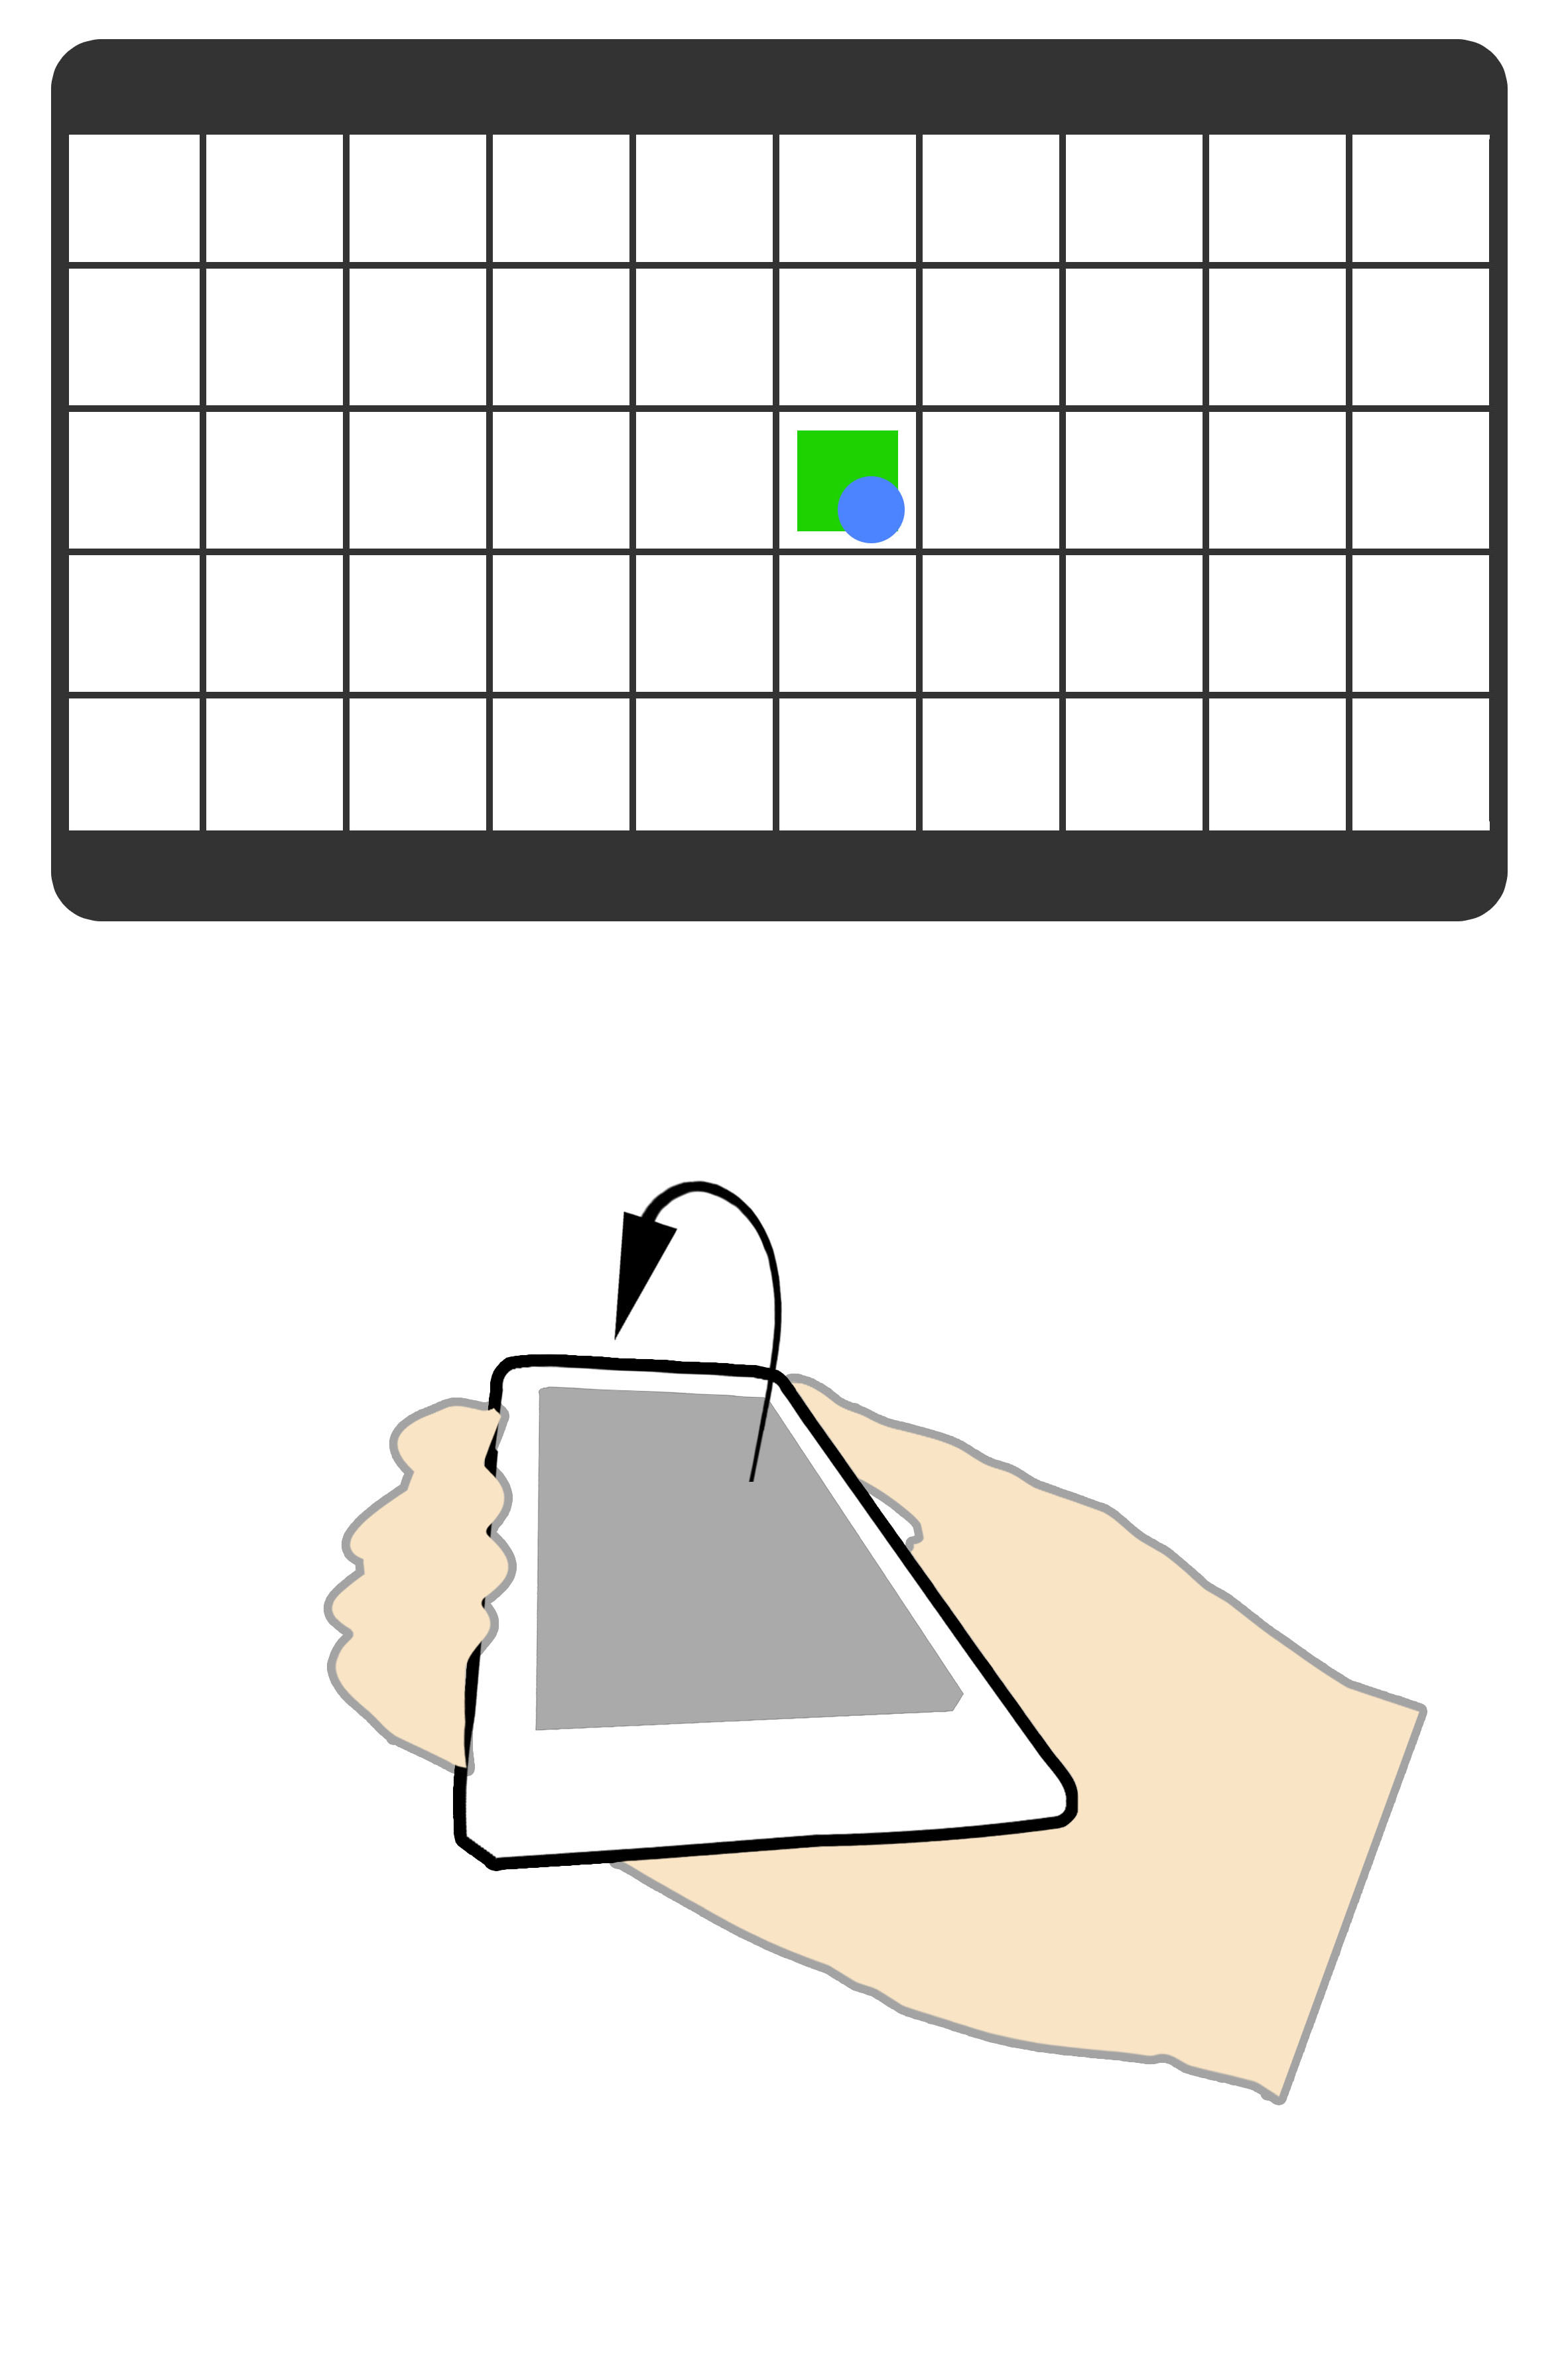
\includegraphics[width = 0.33\columnwidth]{images/techniques/tiltPush3.jpg}\label{fig:tiltPush3}}
	\caption{\push \grab technique}
	\label{fig:grabTechnique}
\end{figure}